\documentclass[sectionlevel=book]{noteformyself}


%一些常用的宏定义
\newcommand{\bbc}{{\mathbb{C}}}
\newcommand{\bbr}{\mathbb{R}}
\newcommand{\bbq}{\mathbb{Q}}
\newcommand{\bbz}{\mathbb{Z}}
\newcommand{\bbn}{\mathbb{N}}
\newcommand{\bbd}{\mathbb{D}}
\newcommand{\bbh}{\mathbb{H}}
\newcommand{\bba}{\mathbb{A}}
\newcommand{\bbp}{\mathbb{P}}
\newcommand{\bbf}{\mathbb{F}}


\newcommand{\ten}{\otimes}
\newcommand{\Var}{\mathbf{Var}}


\newcommand{\calo}{\mathcal{O}}
\newcommand{\cali}{\mathcal{I}}


\newcommand{\fraka}{{\mathfrak{a}}}
\newcommand{\frakm}{{\mathfrak{m}}}
\newcommand{\frakp}{{\mathfrak{p}}}


\newcommand{\Frac}{\mathrm{Frac}}
\newcommand{\Der}{\operatorname{Der}}
\newcommand{\Spec}{\operatorname{Spec}}
\newcommand{\spec}{\operatorname{Spec}}
\newcommand{\mSpec}{\operatorname{mSpec}}
\newcommand{\depth}{\operatorname{depth}}
\newcommand{\idealht}{\operatorname{ht}}
\newcommand{\codim}{\operatorname{codim}}
\newcommand{\Supp}{\operatorname{Supp}}
\newcommand{\trdeg}{\operatorname{trdeg}}
\newcommand{\Ass}{\operatorname{Ass}}
\newcommand{\Ann}{\operatorname{Ann}}


\newcommand{\kk}{\mathsf{k}}
\newcommand{\kkk}{\mathbf{k}}
\newcommand{\KK}{\mathsf{K}}
\newcommand{\KKK}{\mathbf{K}}
\newcommand{\rkk}{\kappa} % residue field
\newcommand{\fkk}{\mathscr{K}} % fraction field
\renewcommand{\d}{\mathrm{d}}
\renewcommand{\i}{\mathrm{i}}
\renewcommand{\P}{\partial}


% \renewcommand{\ker}{\mathrm{Ker}\ }
% \newcommand{\ord}{\mathrm{ord}}
% \renewcommand{\hom}{\mathrm{Hom}}
% \renewcommand{\gcd}{\mathrm{g.c.d.}}
% \newcommand{\laplace}{\Delta}
% \newcommand{\lcm}{\mathrm{l.c.m.}}
\newcommand{\mat}[4]{\left( \begin{array}{cc}#1 &#2 \\ #3 &#4\end{array}\right)}
% \renewcommand{\vec}[1]{\boldsymbol{#1}}
% \renewcommand{\proofname}{\indent\it Proof}




\newcommand{\contradiction}{
    \raisebox{-0.6ex}{\makebox[2.4ex][c]{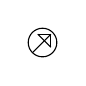
\begin{tikzpicture}
        \draw (0,0) circle (1.2ex);
        \draw (0.7 ex, 0.7 ex) -- (-0.4 ex, 0.7 ex);
        \draw (-0.4 ex, 0.7 ex) -- (0.7 ex, -0.4 ex);
        \draw (0.7 ex, -0.4 ex) -- (0.7 ex, 0.7 ex);
        \draw (0.7 ex, 0.7 ex) -- (-0.848 ex, -0.848 ex);
    \end{tikzpicture}}}
    \ \ 
}

% legendre符号
\makeatletter
\def\legendre@dash#1#2{\hb@xt@#1{%
  \kern-#2\p@
  \cleaders\hbox{\kern.5\p@
    \vrule\@height.2\p@\@depth.2\p@\@width\p@
    \kern.5\p@}\hfil
  \kern-#2\p@
  }}
\def\@legendre#1#2#3#4#5{\mathopen{}\left(
  \sbox\z@{$\genfrac{}{}{0pt}{#1}{#3#4}{#3#5}$}%
  \dimen@=\wd\z@
  \kern-\p@\vcenter{\box0}\kern-\dimen@\vcenter{\legendre@dash\dimen@{#2}}\kern-\p@
  \right)\mathclose{}}
\newcommand\legendre[2]{\mathchoice
  {\@legendre{0}{1}{}{#1}{#2}}
  {\@legendre{1}{.5}{\vphantom{1}}{#1}{#2}}
  {\@legendre{2}{0}{\vphantom{1}}{#1}{#2}}
  {\@legendre{3}{0}{\vphantom{1}}{#1}{#2}}
}
\def\dlegendre{\@legendre{0}{1}{}}
\def\tlegendre{\@legendre{1}{0.5}{\vphantom{1}}}
\makeatother
\addbibresource{Accessories/ref.bib}
\newcommand{\Yang}[1]{\textcolor{red}{#1}}


\title{Notes in Algebraic Geometry}
\author{Tianle Yang}
\date{\today}
\authoremail{\href{mailto:loveandjustice@88.com}{loveandjustice@88.com}}
\authorpage{\href{https://www.tianleyang.com}{www.tianleyang.com}}
\texsource{\href{https://github.com/MonkeyUnderMountain/Note_on_Algebraic_Geometry}{github.com/MonkeyUnderMountain/Note\_on\_Algebraic\_Geometry}}
\version{0.1.0}

\setCJKfamilyfont{lxgwwenkai}{LXGW WenKai} % 定义霞鹜文楷,若未安装,请去掉相关代码编译或使用其他字体
\coversentence{\CJKfamily{lxgwwenkai}「あんたバかァ?」}
\coverimage{Asuka.png} % 封面图片
\coverlinecolor{brown!80!yellow} % 封面横线颜色
\covertitlefont{Allura} % 封面标题字体, 若未安装,可注释掉此行编译或使用其他字体
\covertextcolor{red!80!black} % 封面标题颜色


\begin{document}

    % \pagestyle{empty}
    \maketitle

    \frontmatter

    \tableofcontents

    \mainmatter

    \chapter{Schemes and Varieties}
        \section{Locally Ringed Space}

\subsection{Locally Ringed Space}

    \begin{definition}\label{def:sheaves}
        Let \(X\) be a topological space.
        A \emph{presheaf} of sets (resp. abelian groups, rings, etc.) on \(X\) is a contravariant functor \(\calF : \Open(X) \to \Set\) (resp. \(\Ab\), \(\Ring\), etc.), 
        where \(\Open(X)\) is the category of open subsets of \(X\) with inclusions as morphisms.

        A presheaf \(\calF\) is a \emph{sheaf} if sections can be glued uniquely.
        More precisely, for every open covering \(\{U_i\}_{i \in I}\) of an open set \(U \subset X\) and every family of sections \(s_i \in \calF(U_i)\) such that \(s_i|_{U_i \cap U_j} = s_j|_{U_i \cap U_j}\) for all \(i,j \in I\),
        there exists a unique section \(s \in \calF(U)\) such that \(s|_{U_i} = s_i\) for all \(i \in I\).
    \end{definition}

    \begin{example}\label{eg:sheaf_of_smooth_and_analytic_functions}
        Let \(X\) be a real (resp. complex) manifold.
        The assignment \(U \mapsto C^\infty(U, \bbR)\) (resp. \(U \mapsto \{\text{holomorphic functions on }U\}\)) defines a sheaf of rings on \(X\).
    \end{example}

    \begin{example}\label{eg:presheaf_but_not_sheaf}
        Let \(X\) be a non-connected topological space.
        The assignment 
        \[U \mapsto \{\text{constant functions on }U\}\] 
        defines a presheaf \(\calC\) of rings on \(X\) but not a sheaf.

        For a concrete example, let \(X = (0,1)\cup (2,3)\) with the subspace topology from \(\bbR\).
        Consider the open covering \(\{(0,1), (2,3)\}\) of \(X\).
        The sections \(s_1 = 1 \in \calC((0,1))\) and \(s_2 = 2 \in \calC((2,3))\) agree on the intersection (which is empty), 
        but there is no global section \(s \in \calC(X)\) such that \(s|_{(0,1)} = s_1\) and \(s|_{(2,3)} = s_2\).
    \end{example}

    \begin{definition}\label{def:locally_ringed_space}
        A \emph{locally ringed space} is a pair \((X, \calO_X)\) where \(X\) is a topological space and \(\calO_X\) is a sheaf of rings on \(X\) such that for every \(x \in X\), the stalk \(\calO_{X,x}\) is a local ring.
        
        A \emph{morphism of locally ringed spaces} \(f : (X, \calO_X) \to (Y, \calO_Y)\) consists of a continuous map \(f : X \to Y\) and a morphism of sheaves of rings \(f^\sharp : \calO_Y \to f_*\calO_X\) 
        such that for every \(x \in X\), the induced map on stalks \(f_x^\sharp : \calO_{Y,f(x)} \to \calO_{X,x}\) is a local homomorphism, 
        i.e., it maps the maximal ideal of \(\calO_{Y,f(x)}\) to the maximal ideal of \(\calO_{X,x}\).
    \end{definition}

    \begin{example}\label{eg:non_local_homomorphism_of_local_rings}
        Let \(p\) be a prime number.
        Then the inclusion \(\bbZ_{(p)} \to \bbQ\) is a homomorphism of local rings but not a local homomorphism.
        Here \(\bbZ_{(p)}\) is the localization of \(\bbZ\) at the prime ideal \((p)\).
    \end{example}

    \begin{example}[Glue morphisms]\label{eg:glue_morphisms_of_locally_ringed_spaces}
        Let \(f : (X, \calO_X) \to (Y, \calO_Y)\) be a morphism of locally ringed spaces.
        If \(U \subset X\) and \(V \subset Y\) are open subsets such that \(f(U) \subset V\), then the restriction \(f|_U : (U, \calO_X|_U) \to (V, \calO_Y|_V)\) is a morphism of locally ringed spaces.
        Conversely, if \(\{U_i\}_{i \in I}\) is an open covering of \(X\) and for each \(i \in I\), we have a morphism \(f_i : (U_i, \calO_X|_{U_i}) \to (Y, \calO_Y)\) such that \(f_i|_{U_i \cap U_j} = f_j|_{U_i \cap U_j}\) for all \(i,j \in I\),
        then there exists a unique morphism \(f : (X, \calO_X) \to (Y, \calO_Y)\) such that \(f|_{U_i} = f_i\) for all \(i \in I\).
    \end{example}

    \begin{example}[Glue locally ringed space]\label{eg:glue_open_locally_ringed_subspace}
        We construct a locally ringed space by gluing open subspaces.
        Let \((X_i, \calO_{X_i})\) be locally ringed spaces for \(i \in I\) and \((U_{ij}, \calO_{X_i}|_{U_{ij}})\) be open subspaces for \(i,j \in I\).
        Suppose we have isomorphisms \(\varphi_{ij} : (U_{ij}, \calO_{X_i}|_{U_{ij}}) \to (U_{ji}, \calO_{X_j}|_{U_{ji}})\) such that
        \begin{enumerate}
            \item \(\varphi_{ii} = \id_{X_i}\) for all \(i \in I\);
            \item \(\varphi_{ij}(U_{ij} \cap U_{ik}) = U_{ji} \cap U_{jk}\) for all \(i,j \in I\);
            \item \(\varphi_{jk}\circ \varphi_{ij} = \varphi_{ik}\) on \(U_{ij} \cap U_{ik}\) for all \(i,j,k \in I\).
        \end{enumerate}
        Then there exists a locally ringed space \((X, \calO_X)\) and open immersions \(\psi_i : (X_i, \calO_{X_i}) \to (X, \calO_X)\) uniquely up to isomorphism such that 
        \begin{enumerate}
            \item \(\varphi_i(U_{ij}) = \psi_i(X_i)\cap \psi_j(X_j)\) for all \(i,j \in I\);
            \item the following diagram 
                \[ \begin{tikzcd}
                    (U_{ij}, \calO_{X_i}|_{U_{ij}}) \arrow[d, "\varphi_{ij}"'] \arrow[r, hook] & (X_i, \calO_{X_i}) \arrow[r, hook, "\psi_i"] & (X, \calO_X) \arrow[d, "="] \\
                    (U_{ji}, \calO_{X_j}|_{U_{ji}}) \arrow[r, hook] & (X_j, \calO_{X_j}) \arrow[r, hook, "\psi_j"] & (X, \calO_X)
                \end{tikzcd} \]
                commutes for all \(i,j \in I\);
            \item \(X = \bigcup_{i \in I} \psi_i(X_i)\).
        \end{enumerate}
        Such \((X, \calO_X)\) is called \emph{the locally ringed space obtained by gluing the \((X_i, \calO_{X_i})\) along the \(\varphi_{ij}\)}.
        
        First \(\varphi_{ij}\) induces an equivalence relation \(\sim\) on the disjoint union \(\coprod_{i \in I} X_i\).
        By taking the quotient space, we can glue the underlying topological spaces to get a topological space \(X\).
        The structure sheaf \(\calO_X\) is given by 
        \[ \calO_X(V) := \left\{ (s_i)_{i \in I} \in \prod_{i \in I} \calO_{X_i}(\psi_i^{-1}(V)) \;\middle|\; s_i|_{U_{ij}} = \varphi_{ij}^\sharp(s_j|_{U_{ji}}) \text{ for all } i,j \in I \right\}. \]
        Easy to check that \((X, \calO_X)\) is a locally ringed space and satisfies the required properties.
        If there is another locally ringed space \((X', \calO_{X'})\) with \(\psi'_i\) satisfying the same properties, then by gluing \(\psi_i' \circ \psi_i^{-1}\) we get an isomorphism \((X, \calO_X) \to (X', \calO_{X'})\).
    \end{example}

        \section{Definition and First Properties}


\subsection{Locally Ringed Space}


\subsection{Schemes}

    \begin{example}[Glue open subschemes]\label{eg:glue_open_subschemes}
        We construct a scheme by gluing open subschemes.
        Let \(X_i\) be schemes for \(i \in I\) and \(U_{ij} \subseteq X_i\) be open subschemes for \(i,j \in I\).
        Suppose we have isomorphisms \(\varphi_{ij} : U_{ij} \to U_{ji}\) such that
        \begin{enumerate}
            \item \(\varphi_{ii} = \id_{X_i}\) for all \(i \in I\);
            \item \(\varphi_{ij}(U_{ij} \cap U_{ik}) = U_{ji} \cap U_{jk}\) for all \(i,j \in I\);
            \item \(\varphi_{jk}\circ \varphi_{ij} = \varphi_{ik}\) on \(U_{ij} \cap U_{ik}\) for all \(i,j,k \in I\).
        \end{enumerate}
        \Yang{}
    \end{example}

        \section{Category of sheaves of modules}

\subsection{Sheaves of modules, quasi-coherent and coherent sheaves}

    \begin{definition}\label{def:sheaf_of_modules}
        Let $X$ be a ringed space with structure sheaf $\calO_X$. A \textbf{sheaf of (left) $\calO_X$-modules} is a sheaf $\calF$ on $X$ such that for every open set $U\subseteq X$, $\calF(U)$ is an $\calO_X(U)$-module, and for every inclusion of open sets $V\subseteq U$, the restriction map $\rho_{UV}:\calF(U)\to \calF(V)$ is compatible with the restriction map $\rho_{UV}:\calO_X(U)\to \calO_X(V)$ in the sense that for every $s\in \calO_X(U)$ and $m\in \calF(U)$, we have
        \[
            \rho_{UV}(s\cdot m) = \rho_{UV}(s)\cdot \rho_{UV}(m).
        \]
        \Yang{To be continued...}
    \end{definition}

    \begin{example}\label{eg:module_as_sheaf_of_modules_in_affine_case}
        Let $X$ be a scheme. The structure sheaf $\calO_X$ is a sheaf of $\calO_X$-modules. More generally, any quasi-coherent sheaf (to be defined later) is a sheaf of $\calO_X$-modules.
        In particular, if $X=\Spec A$ is an affine scheme, then for any $A$-module $M$, the associated sheaf $\widetilde{M}$ is a sheaf of $\calO_X$-modules.
        \Yang{To be continued...}
    \end{example}

    \begin{definition}\label{def:quasi-coherent_sheaf}
        Let $X$ be a scheme. A sheaf of $\calO_X$-modules $\calF$ is called \textbf{quasi-coherent} if for every point $x\in X$, there exists an open neighborhood $U$ of $x$ such that $\calF|_U$ is isomorphic to the cokernel of a morphism of free $\calO_U$-modules, i.e., there exists an exact sequence of sheaves of $\calO_U$-modules
        \[
            \calO_U^{(I)} \to \calO_U^{(J)} \to \calF|_U \to 0,
        \]
        where $I,J$ are (possibly infinite) index sets.
        \Yang{To be continued...}
    \end{definition}

    \begin{definition}\label{def:coherent_sheaf}
        Let $X$ be a scheme. A sheaf of $\calO_X$-modules $\calF$ is called \textbf{coherent} if it is quasi-coherent and for every point $x\in X$, there exists an open neighborhood $U$ of $x$ such that $\calF|_U$ is isomorphic to the cokernel of a morphism of finite free $\calO_U$-modules, i.e., there exists an exact sequence of sheaves of $\calO_U$-modules
        \[
            \calO_U^m \to \calO_U^n \to \calF|_U \to 0,
        \]
        where $m,n$ are finite integers.
        \Yang{To be continued...}
    \end{definition}

\subsection{As abelian categories}

    \begin{theorem}\label{thm:category_of_sheaves_of_modules_is_abelian}
        Let $X$ be a ringed space. The category of sheaves of $\calO_X$-modules is an abelian category.
        \Yang{To be continued...}
    \end{theorem}

    \begin{theorem}\label{thm:category_of_quasi-coherent_sheaves_is_abelian}
        Let $X$ be a scheme. The category of quasi-coherent sheaves on $X$ is an abelian category.
        \Yang{To be continued...}
    \end{theorem}

    \begin{theorem}\label{thm:category_of_coherent_sheaves_is_abelian}
        Let $X$ be a noetherian scheme. The category of coherent sheaves on $X$ is an abelian category.
        \Yang{To be continued...}
    \end{theorem}

\subsection{Relevant functors}

    \begin{theorem}\label{thm:global_sections_functor}
        Let $X$ be a ringed space. The global sections functor
        \[
            \Gamma(X,-): \text{(Sheaves of $\calO_X$-modules)} \to \text{($\calO_X(X)$-modules)}
        \]
        is left exact.
        \Yang{To be continued...}
    \end{theorem}

    \begin{theorem}\label{thm:direct_image_functor}
        Let $f:X\to Y$ be a morphism of ringed spaces. The direct image functor
        \[
            f_*: \text{(Sheaves of $\calO_X$-modules)} \to \text{(Sheaves of $\calO_Y$-modules)}
        \]
        is left exact.
        \Yang{To be continued...}
    \end{theorem}

    \begin{theorem}\label{thm:inverse_image_functor}
        Let $f:X\to Y$ be a morphism of ringed spaces. The inverse image functor
        \[
            f^*: \text{(Sheaves of $\calO_Y$-modules)} \to \text{(Sheaves of $\calO_X$-modules)}
        \]
        is right exact.
        \Yang{To be continued...}
    \end{theorem}

\subsection{Locally free sheaves and vector bundles}

    \begin{definition}\label{def:locally_free_sheaf}
        Let $X$ be a scheme. A sheaf of $\calO_X$-modules $\calF$ is called \textbf{locally free} if for every point $x\in X$, there exists an open neighborhood $U$ of $x$ such that $\calF|_U$ is isomorphic to a finite free $\calO_U$-module, i.e., there exists an isomorphism of sheaves of $\calO_U$-modules
        \[
            \calF|_U \cong \calO_U^n,
        \]
        where $n$ is a finite integer called the \textbf{rank} of $\calF$ at $x$.
        \Yang{To be continued...}
    \end{definition}

    \begin{example}\label{eg:line_bundle}
        A \textbf{line bundle} on a scheme $X$ is a locally free sheaf of rank 1. The sheaf of differentials $\Omega_{X/k}$ on a smooth variety $X$ over a field $k$ is a locally free sheaf of rank equal to the dimension of $X$.
        \Yang{To be continued...}
    \end{example}

    \begin{theorem}\label{thm:locally_free_sheaf_is_vector_bundle}
        Let $X$ be a scheme. There is an equivalence of categories between the category of locally free sheaves of finite rank on $X$ and the category of vector bundles on $X$.
        \Yang{To be continued...}
    \end{theorem}

\subsection{Cohomological theory}

    \begin{theorem}\label{thm:cohomology_of_sheaves_of_modules}
        Let $X$ be a ringed space and $\calF$ a sheaf of $\calO_X$-modules. Then the cohomology groups $H^i(X,\calF)$ are $\calO_X(X)$-modules for all $i\geq 0$.
        \Yang{To be continued...}
    \end{theorem}

    \begin{theorem}\label{thm:cohomology_of_quasi-coherent_sheaves}
        Let $X$ be a scheme and $\calF$ a quasi-coherent sheaf on $X$. Then the cohomology groups $H^i(X,\calF)$ are $\calO_X(X)$-modules for all $i\geq 0$.
        \Yang{To be continued...}
    \end{theorem}

    \begin{theorem}\label{thm:cohomology_of_coherent_sheaves}
        Let $X$ be a noetherian scheme and $\calF$ a coherent sheaf on $X$. Then the cohomology groups $H^i(X,\calF)$ are $\calO_X(X)$-modules for all $i\geq 0$.
        \Yang{To be continued...}
    \end{theorem}
        \section{Line Bundles and Divisors}

\subsection{Cartier Divisors}

\subsection{Line Bundles and Picard Group}

    \begin{definition}\label{def:picard_group}
        Let \(X\) be a scheme. 
        The \emph{Picard group} of \(X\) is defined to be \(\Pic(X) = H^1(X, \calO_X^*)\).
        The group operation is given by the tensor product of line bundles.
    \end{definition}

    \begin{definition}\label{def:algebraically_equivalent_line_bundles}
        Let \(X\) be a scheme over a field \(\kk\) and \(\calL, \calL'\) two line bundles on \(X\).
        We say that \(\calL\) and \(\calL'\) are \emph{algebraically equivalent} if there exists a \Yang{non-singular} variety \(T\) over \(\kk\), two points \(t_0, t_1 \in T(\kkk)\) and a line bundle \(\calM\) on \(X \times T\) such that 
        \[ \calM|_{X \times \{t_0\}} \cong \calL, \quad \calM|_{X \times \{t_1\}} \cong \calL'. \]
        We denote it by \(\calL \sim_{\text{alg}} \calL'\).
        \Yang{To be checked.}
    \end{definition}

\subsection{Weil Divisors and Reflexive Sheaves}

        \section{Line bundles induce morphisms}


\subsection{Ample and basepoint free line bundles}

    The story begins with the following theorem, which uses global sections of a line bundle to construct a morphism to projective space.

    \begin{theorem}\label{thm:morphism_to_projective_space}
        Let \(A\) be a ring and \(X\) an \(A\)-scheme.
        Let \(\calL\) be a line bundle on \(X\) and \(s_0,\ldots,s_n\in\Gamma(X,\calL)\).
        Suppose that \(\{s_i\}\) generate \(\calL\), i.e., \(\bigoplus_i \calO_X\cdot s_i \to \calL\) is surjective.
        Then there is a unique morphism \(f:X\to \bbP^n_A\) such that \(\calL\cong f^*\calO(1)\) and \(s_i=f^*x_i\), where \(x_i\) are the standard coordinates on \(\bbP^n_A\).   
    \end{theorem}
    \begin{proof}
        Let \(U_i\coloneqq \{\xi \in X: s_i(\xi) \not\in \frakm_\xi \calL_\xi\}\) be the open subset where \(s_i\) does not vanish.
        Since \(\{s_i\}\) generate \(\calL\), we have \(X=\bigcup_i U_i\).
        Let \(V_i\) be given by \(x_i \neq 0\) in \(\bbP^n_A\).
        On \(U_i\), let \(f_i:U_i\to V_i \subseteq \bbP^n_A\) be the morphism induced by the ring homomorphism
        \[ A\left[\frac{x_0}{x_i},\ldots,\frac{x_n}{x_i}\right] \to \Gamma(U_i,\calO_X), \quad \frac{x_j}{x_i} \mapsto \frac{s_j}{s_i}. \]
        Easy to check that on \(U_i\cap U_j\), \(f_i\) and \(f_j\) agree.
        Thus we can glue them to get a morphism \(f:X\to \bbP^n_A\).
        By construction, we have \(s_i=f^*x_i\) and \(\calL\cong f^*\calO(1)\).
        If there is another morphism \(g:X\to \bbP^n_A\) satisfying the same properties, then on each \(U_i\), \(g\) must agree with \(f_i\) by the same construction.
        Thus \(g=f\).
    \end{proof}

    \begin{proposition}\label{prop:different_choices_of_sections_give_different_morphisms_which_differ_by_a_linear_transformation}
        Let \(X\) be a \(\kk\)-scheme for some field \(\kk\) and \(\calL\) is a line bundle on \(X\).
        Suppose that \(\{s_0,\ldots,s_n\}\) and \(\{t_0,\ldots,t_m\}\) span the same subspace \(V\subseteq \Gamma(X,\calL)\) and both generate \(\calL\).
        Let \(f:X\to \bbP^n_\kk\) and \(g:X\to \bbP^m_\kk\) be the morphisms induced by \(\{s_i\}\) and \(\{t_j\}\) respectively.
        Then there exists a linear transformation \(\phi:\bbP^n_\kk \ratmap \bbP^m_\kk\) which is well defined near image of \(f\) and satisfies \(g=\phi \circ f\).
    \end{proposition}
    \begin{proof}
        
    \end{proof}

    \begin{example}\label{eg:d-uple_embedding_or_Veronese_embedding}
        Let \(X=\bbP^n_\kk\) with \(\kk\) a field and \(\calL=\calO_{\bbP^n}(d)\) for some \(d>0\).
        Then \(\Gamma(X,\calL)\) is generated by the global sections \(S_{i_0,\ldots,i_n}=T_0^{i_0}T_1^{i_1}\cdots T_n^{i_n}\) for all \((i_0,\ldots,i_n)\) with \(i_0+\cdots+i_n=d\), where \(T_i\) are the standard coordinates on \(\bbP^n\).
        The they induce a morphism \(f:X\to \bbP^N_\kk\) where \(N=\binom{n+d}{d}-1\).
        On \(\kk\)-point level, it is given by
        \[
            [x_0:\cdots:x_n] \mapsto [\ldots:x_0^{i_0}x_1^{i_1}\cdots x_n^{i_n}:\ldots],
        \]
        where the coordinates on the right-hand side are indexed by all \((i_0,\ldots,i_n)\) with \(i_0+\cdots+i_n=d\).
        This is called the \emph{\(d\)-uple embedding} or \emph{Veronese embedding} of \(\bbP^n\) into \(\bbP^N\).
    \end{example}

    \begin{example}\label{eg:Segre_embedding}
        Let \(X=\bbP^m_\kk \times \bbP^n_\kk\) with \(\kk\) a field and \(\calL=\pi_1^*\calO_{\bbP^m}(1) \otimes \pi_2^*\calO_{\bbP^n}(1)\), where \(\pi_1\) and \(\pi_2\) are the projections.
        Let \(T_0,\ldots,T_m\) and \(S_0,\ldots,S_n\) be the standard coordinates on \(\bbP^m\) and \(\bbP^n\) respectively.
        Then \(\Gamma(X,\calL)\) is generated by the global sections \(T_i S_j = \pi_1^*T_i \otimes \pi_2^*S_j\) for \(0\leq i \leq m\) and \(0\leq j \leq n\).
        They induce a morphism \(f:X\to \bbP^{(m+1)(n+1)-1}_\kk\).
        On \(\kk\)-point level, it is given by
        \[ ([x_0:\cdots:x_m],[y_0:\cdots:y_n]) \mapsto [\ldots:x_i y_j:\ldots], \]
        where the coordinates on the right-hand side are indexed by all \((i,j)\) with \(0\leq i \leq m\) and \(0\leq j \leq n\).
        This is called the \emph{Segre embedding} of \(\bbP^m \times \bbP^n\) into \(\bbP^{(m+1)(n+1)-1}\).
    \end{example}

    \begin{example}\label{eg:morphism_induced_by_-K_of_Hirzebruch_surface_F_2}
        Let \(X=\bbF_2\) be the second Hirzebruch surface, i.e., the projective bundle \(\bbP_{\bbP^1}(\calO_{\bbP^1}\oplus \calO_{\bbP^1}(-2))\) over \(\bbP^1\).
        \Yang{To be continued.}
    \end{example}


    \begin{definition}\label{def:ample_line_bundle}
        A line bundle \(\calL\) on a scheme \(X\) is \emph{ample} if for every coherent sheaf \(\calF\) on \(X\), there exists \(n_0>0\) such that for all \(n\ge n_0\), \(\calF\otimes \calL^{\otimes n}\) is globally generated.
        \Yang{To be continued.}
    \end{definition}

    \begin{definition}\label{def:very_ample_line_bundle}
        A line bundle \(\calL\) on a scheme \(X\) is \emph{very ample} if there exists a closed embedding \(i:X\to \bbP^n_A\) such that \(\calL\cong i^*\calO(1)\).
        \Yang{To be continued.}
    \end{definition}

    \begin{definition}\label{def:base_locus}
        Let \(\calL\) be a line bundle on a scheme \(X\) and \(V\subseteq \Gamma(X,\calL)\) a subspace.
        The \emph{base locus} of \(V\) is the closed subset
        \[
            \Bs(V) = \{x\in X : s(x)=0, \forall s\in V\}.
        \]
        If \(\Bs(V)=\emptyset\), we say that \(V\) is \emph{base-point free}.
        \Yang{To be continued.}
    \end{definition}

    \begin{definition}\label{def:globally_generated_line_bundle}
        A line bundle \(\calL\) on a scheme \(X\) is \emph{globally generated} if \(\Gamma(X,\calL)\) generates \(\calL\), i.e., the natural map \(\Gamma(X,\calL)\otimes \calO_X \to \calL\) is surjective.
        \Yang{To be continued.}
    \end{definition}

    \begin{definition}\label{def:base_locus_and_base_idea}
        Let \(\calL\) be a line bundle on a scheme \(X\).
        \Yang{To be continued.}
    \end{definition}

    % \begin{definition}\label{def:linear_system}
    %     A \emph{linear system} on a scheme \(X\) is a pair \((\calL,V)\) where \(\calL\) is a line bundle on \(X\) and \(V\subseteq \Gamma(X,\calL)\) is a subspace.
    %     The dimension of the linear system is \(\dim V - 1\).
    %     A linear system is \emph{base-point free} if \(V\) is base-point free.
    %     A linear system is \emph{complete} if \(V=\Gamma(X,\calL)\).
    %     \Yang{To be continued.}
    % \end{definition}

    \begin{theorem}\label{thm:ample_very_ample}
        Let \(X\) be a scheme over a ring \(A\) and \(\calL\) a line bundle on \(X\).
        Then the following are equivalent:
        \begin{enumerate}
            \item \(\calL\) is ample;
            \item for some \(n>0\), \(\calL^{\otimes n}\) is very ample.
            % \item suppose that \(X\) is of fibFor all \(n \gg 0\), \(\calL^{\otimes n}\) is very ample.
        \end{enumerate}
        If furthermore \(X\) is of finite type over noetherian ring \(A\), then the above are also equivalent to:
        \begin{enumerate}
            \item[(c)] for all \(n \gg 0\), \(\calL^{\otimes n}\) is very ample.
        \end{enumerate}
        \Yang{To be continued.}
    \end{theorem}

    \begin{proposition}\label{prop:tensor_with_ample_very_ample_and_bpf}
        
    \end{proposition}

\subsection{Linear systems}

    In this subsection, we give a more geometric interpretation of last subsection using the language of linear systems.

    \begin{definition}\label{def:complete_linear_system}
        Let \(X\) be a normal proper variety over a field \(\kk\), \(D\) a (Cartier) divisor on \(X\) and \(\calL=\calO_X(D)\) the associated line bundle.
        The \emph{complete linear system} associated to \(D\) is the set 
        \[ |D| = \{D'\in \CaDiv(X) : D'\sim D, D' \geq 0\}. \]
    \end{definition}

    There is a natural bijection between the complete linear system \(|D|\) and the projective space \(\bbP(\Gamma(X,\calL))\).
    Here the elements in \(\bbP(\Gamma(X,\calL))\) are one-dimensional subspaces of \(\Gamma(X,\calL)\).
    Consider the vector subspace \(V\subseteq \Gamma(X,\calL)\), we can define the generate linear system \(|V|\) as the image of \(V\setminus \{0\}\) in \(\bbP(\Gamma(X,\calL))\).

\subsection{Asymptotic behavior}

    \begin{definition}\label{def:section_ring}
        Let \(X\) be a scheme and \(\calL\) a line bundle on \(X\).
        The \emph{section ring} of \(\calL\) is the graded ring
        \[
            R(X,\calL) = \bigoplus_{n\ge 0} \Gamma(X,\calL^{\otimes n}),
        \]
        with multiplication induced by the tensor product of sections.
        \Yang{To be continued.}
        
    \end{definition}

    \begin{definition}\label{def:semiample_line_bundle}
        A line bundle \(\calL\) on a scheme \(X\) is \emph{semiample} if for some \(n>0\), \(\calL^{\otimes n}\) is base-point free.
        \Yang{To be continued.}
        
    \end{definition}

    \begin{theorem}\label{thm:fibration_associated_to_semiample_line_bundle}
        Let \(X\) be a scheme over a ring \(A\) and \(\calL\) a semiample line bundle on \(X\).
        Then there exists a morphism \(f:X\to Y\) over \(A\) such that \(\calL\cong f^*\calO_Y(1)\) for some very ample line bundle \(\calO_Y(1)\) on \(Y\).
        Moreover, \(Y=\Proj R(X,\calL)\) and \(f\) is induced by the natural map \(R(X,\calL)\to \Gamma(X,\calL^{\otimes n})\).
        \Yang{To be continued.  }
        
    \end{theorem}

    \begin{definition}\label{def:big_line_bundle}
        A line bundle \(\calL\) on a scheme \(X\) is \emph{big} if the section ring \(R(X,\calL)\) has maximal growth, i.e., there exists \(C>0\) such that
        \[
            \dim \Gamma(X,\calL^{\otimes n}) \ge C n^{\dim X}
        \]
        for all sufficiently large \(n\).
        \Yang{To be continued.}
        
    \end{definition}

    \begin{example}\label{eg:base_locus_-K_of_Hirzebruch_surface}
        Let \(X=\bbF_2\) be the second Hirzebruch surface, i.e., the projective bundle \(\bbP(\calO_{\bbP^1}\oplus \calO_{\bbP^1}(2))\) over \(\bbP^1\).
        Let \(\pi:X\to \bbP^1\) be the projection and \(E\) the unique section of \(\pi\) with self-intersection \(-2\).
        Then the anticanonical bundle \(-K_X\) is big but not base-point free.
        In fact, we have
        \[
            K_X = -2E - 4F,
        \]
        where \(F\) is a fiber of \(\pi\).
        Thus
        \[
            -K_X = 2E + 4F.
        \]
        Since \(E^2=-2<0\), any section of \(-K_X\) must vanish on \(E\).
        Thus \(E\subseteq \Bs(-K_X)\), so \(-K_X\) is not base-point free.
        On the other hand, we have
        \[
            H^0(X,\calO_X(-nK_X)) = H^0(X,\calO_X(2nE + 4nF)).
        \]
        Using the projection formula and the fact that \(\pi_*\calO_X(E) = \calO_{\bbP^1} \oplus \calO_{\bbP^1}(-2)\), we can compute that
        \[
            H^0(X,\calO_X(2nE + 4nF)) = H^0(\bbP^1, S^{2n}(\calO_{\bbP^1} \oplus \calO_{\bbP^1}(-2)) \otimes \calO_{\bbP^1}(4n)).
        \]
        The right-hand side can be computed to be a direct sum of line bundles on \(\bbP^1\), and for large \(n\), it contains many global sections.
        In fact, one can show that
        \[
            \dim H^0(X,\calO_X(-nK_X)) \sim 4n^2 \text{ for large } n,
        \]
        \Yang{To be continued.}
        
    \end{example}


% \subsection{Iitaka fibration}

%     \begin{theorem}\label{thm:Iitaka_fibration}
%         Let \(X\) be a projective variety over a field \(k\) and \(\calL\) a line bundle on \(X\).
%         Then there exists a unique rational map \(f:X\dashrightarrow Y\) to a projective variety \(Y\) such that:
%         \begin{enumerate}
%             \item The general fiber of \(f\) is connected.
%             \item The dimension of \(Y\) is equal to the Iitaka dimension of \(\calL\), i.e., the transcendence degree of the section ring \(R(X,\calL)\) minus one.
%             \item For some \(n>0\), the linear system associated to \(\calL^{\otimes n}\) defines the map \(f\).
%         \end{enumerate}
%         The map \(f\) is called the \emph{Iitaka fibration} associated to \(\calL\).
%         \Yang{To be continued.}
        
%     \end{theorem}

    \chapter{More Scattered Topics}

    \chapter{Surfaces}
        \section{The first properties of surfaces}

Let \(\kkk\) be an algebraically closed field of arbitrary characteristic.
Unless otherwise specified, all varieties are defined over \(\kkk\).

\subsection{Basic concepts}


\subsection{Riemann-Roch Theorem for surfaces}


\subsection{Hodge Index Theorem}
        \section{}

        \section{}

        \section{Ruled Surface}

In this section, fix an algebraically closed field $\kkk$.

\subsection{Preliminaries}

    Let \(S\) be a variety over \(\kkk\) and \(\calE\) a vector bundle of rank \(r+1\) on \(S\).

    \begin{proposition}\label{prop:isomorphic_projective_bundle_iff_twist_by_line_bundle}
        The \(S\)-varieties \(\bbP_X(\calE) \cong \bbP_X(\calE')\) if and only if \(\calE \cong \calE' \otimes \calL\) for some line bundle \(\calL\) on \(S\).
    \end{proposition}

    \begin{theorem}\label{thm:Eulur_sequence_for_projective_bundle}
        Let \(\pi: X=\bbP_S(\calE) \to S\) be the projective bundle associated to a vector bundle \(\calE\) of rank \(r+1\) on \(S\). 
        Then there is an exact sequence of vector bundles on \(\bbP_S(\calE)\)
        \[
            0 \to \Omega_{\bbP_S(\calE)/S} \to \pi^*(\calE)(-1) \to \calO_{\bbP_S(\calE)} \to 0.
        \]
        In particular, \(K_X \sim \pi^*(K_S + \det \calE) - (r+1)\calO_{\bbP_S(\calE)}(1)\).
        \Yang{To be continued...}
    \end{theorem}

    \begin{theorem}[Tsen's Theorem, {\cite[Tag 03RD]{Stacks}}]\label{thm:Tsen_theorem}
        Let \(C\) be a smooth curve over an algebraically closed field \(\kkk\). 
        Then \(\KK=\kkk(C)\) is a \(C_1\) field, i.e., every degree \(d\) hypersurface in \(\bbP^n_{\KK}\) has a \(\KK\)-rational point provided \(d \leq n\).
        % \Yang{Need a reference.}
    \end{theorem}

    % \begin{theorem}[Cohomology and Base Change, {\cite[Theorem 12.11]{Har77}}]\label{thm:cohomology_and_base_change}
    %     Let \(f:X \to S\) be a projective morphism of noetherian schemes and \(\calF\) a coherent sheaf on \(X\) which is flat over \(S\). 
    %     Then for each \(i \geq 0\) and each point \(s \in S\) there is a natural base change homomorphism
    %     \[
    %         \varphi_s^i: \sfR^i f_*\calF \ten_{\calO_S} \rkk(s) \to H^i(X_s,\calF_s).
    %     \]
    %     Suppose that \(\varphi_s^i\) is surjective. 
    %     Then
    %     \begin{enumerate}
    %         \item there exists an open neighborhood \(U\) of \(s\) such that \(\varphi_{s'}^i\) is an isomorphism for all \(s' \in U\);
    %         \item TFAE:
    %             \begin{enumerate}
    %                 \item \(\varphi_{s}^{i-1}\) is surjective;
    %                 \item \(\sfR^i f_*\calF\) is locally free on an open neighborhood of \(s\).
    %             \end{enumerate}
    %     \end{enumerate}
    % \end{theorem}

    \begin{theorem}[Grauert's Theorem, {\cite[Corollary 12.9]{Har77}}]\label{thm:Grauert_theorem}
        Let \(f:X \to S\) be a projective morphism of noetherian schemes and \(\calF\) a coherent sheaf on \(X\) which is flat over \(S\).
        Suppose that \(S\) is integral and the function \(s \mapsto \dim_{\rkk(s)} H^i(X_s,\calF_s)\) is constant on \(S\) for some \(i \geq 0\). 
        Then \(\sfR^i f_*\calF\) is locally free and the base change homomorphism
        \[
            \varphi_s^i: \sfR^i f_*\calF \ten_{\calO_S} \rkk(s) \to H^i(X_s,\calF_s)
        \]
        is an isomorphism for all \(s \in S\).
    \end{theorem}

    \begin{theorem}[Miracle Flatness, {\cite[Theorem 23.1]{Mat89}}]\label{thm:miracle_flatness}
        Let \(f:X \to Y\) be a morphism of noetherian schemes. 
        Assume that \(Y\) is regular and \(X\) is Cohen-Macaulay. 
        If all fibers of \(f\) have the same dimension \(d = \dim X - \dim Y\), then \(f\) is flat.
    \end{theorem}

    \begin{proposition}[Geometric form of Nakayama's Lemma]\label{prop: geometric form of Nakayama's lemma}
        Let \(X\) be a variety, $x\in X$ a closed point and $\calF$ a coherent sheaf on $X$.
        If $a_1,\cdots,a_k \in \calF(X)$ generate $\calF|_x = \calF \ten \rkk(x)$, then there is an open subset $U \subset X$ such that $a_i|_U$ generate $\calF(U)$. 
    \end{proposition}

    \begin{proposition}\label{prop:relative_projective_morphism}
        Let \(S\) be a noetherian scheme and \(\calE\) a vector bundle of rank \(r+1\) on \(S\). 
        % Then the projection \(\pi:\bbP_X(\calE) \to X\) is a projective morphism.
        Let \(X\) be a \(S\)-scheme via a morphism \(g:X \to S\).
        Then there is a bijection
        \[
            \{S\text{-morphisms } X \to \bbP_S(\calE)\}
            \leftrightarrow
            \left\{
                \begin{array}{l}
                    \text{surjective homomorphisms } g^*\calE \to \calL \\
                    \text{where } \calL \text{ is a line bundle on } X
                \end{array}
            \right\}.
        \]
        \Yang{Need to check.}
    \end{proposition}
    \begin{proof}
        Take an affine cover \(\{U_i\}\) of \(S\) such that \(\calE|_{U_i}\) is trivial.
        On \(U_i\), the surjection \(g^*\calE|_{U_i} \surjmap \calL|_{X_{U_i}}\) gives a morphism \(X_{U_i} \to \bbP_{U_i}(\calE|_{U_i}) \cong \bbP_{S}(\calE)_{U_i}\) by \Yang{ref}.

    \end{proof}

\subsection{Minimal Section and Classification}

    \begin{definition}[Ruled surface]\label{def:ruled_surface}
        A \emph{ruled surface} is a smooth projective surface \(X\) together with a surjective morphism \(\pi:X \to C\) to a smooth curve \(C\) such that all fibers of \(\pi\) are isomorphic to \(\bbP^1\).
    \end{definition}

    Let \(\pi:X \to C\) be a ruled surface over a smooth curve \(C\) of genus \(g\).


    \begin{lemma}\label{lem:existence_of_section_of_ruled_surface}
        There exists a section of \(\pi\).
    \end{lemma}
    \begin{proof}
        \Yang{To be continued...}
    \end{proof}

    \begin{proposition}\label{prop:ruled_surface_as_projective_bundle}
        % Let \(\pi:X \to C\) be a ruled surface over a smooth curve \(C\). 
        Then there exists a vector bundle \(\calE\) of rank \(2\) on \(C\) such that \(X \cong \bbP_C(\calE)\) over \(C\).
    \end{proposition}
    \begin{proof}
        Let \(\sigma:C \to X\) be a section of \(\pi\) and \(D\) be its image.
        Let \(\calL = \calO_X(D)\) and \(\calE = \pi_*\calL\).
        Since \(D\) is a section of \(\pi\), \(\calL|_{X_t} \cong \calO_{\bbP^1}(1)\) for any \(t \in C\), whence \(h^0(X_t,\calL|_{X_t}) = 2\) for any \(t \in C\).
        By Miracle Flatness (\cref{thm:miracle_flatness}), \(f\) is flat.
        By Grauert's Theorem (\cref{thm:Grauert_theorem}), \(\calE\) is a vector bundle of rank \(2\) on \(C\) and we have a natural isomorphism \(\calE \ten \rkk(t) \cong H^0(X_t,\calL|_{X_t})\) for any \(t \in C\).

        This gives a surjective homomorphism 
        \[ \calE \ten_{\calO_C} \rkk(t) \ten_{\rkk(t)} \calO_{X_t} \cong H^0(X_t,\calL|_{X_t}) \ten_{\rkk(t)} \calO_{X_t} \surjmap \calL|_{X_t}. \]
        For every \(x \in X\), we have 
        \[ \calE \ten_{\calO_C} \rkk(\pi(x)) \ten_{\rkk(\pi(x))} \calO_{X_{\pi(x)}} \ten_{\calO_{X_{\pi(x)}}} \rkk(x)  \surjmap \calL|_{X_{\pi(x)}}\ten_{\calO_{X_{\pi(x)}}} \rkk(x). \]
        \Yang{The left side coincides with \(\pi^*\calE\ten_{\calO_X} \rkk(x)\) naturally.}
        Hence by Nakayama's Lemma, the natural homomorphism \(\pi^*\calE \to \calL\) is surjective.

        Denote by \(p: \bbP_C(\calE) \to C\) the projection.
        Take an affine open cover \(\{U_i\}\) of \(C\) such that \(\calE|_{U_i}\) is trivial.
        On \(U_i\), the surjection \(\pi^*\calE|_{X_{U_i}} \surjmap \calL|_{X_{U_i}}\) gives a morphism \(\varphi_i: X_{U_i} \to \bbP_{U_i}(\calE|_{U_i}) \cong \bbP_{C}(\calE)_{U_i}\) by \Yang{ref}.
        Since \(\varphi_i\) and \(\varphi_j\) agree on \(X_{U_i \cap U_j}\), they glue to give a morphism \(\varphi:X \to \bbP_C(\calE)\) over \(C\).
        Since \(\varphi|_{X_t}:X_t \to \bbP_C(\calE)_t\) is an isomorphism for any \(t \in C\), \(\varphi\) is 
        % Since both \(X\) and \(\bbP_C(\calE)\) are smooth, \(\varphi\) is an isomorphism.
    \end{proof}

    \begin{lemma}\label{lem:correspondence_between_sections_and_quotient_line_bundles}
        Fix a vector bundle \(\calE\) of rank \(2\) on \(C\) such that \(X \cong \bbP_C(\calE)\).
        There is a one-to-one correspondence between sections of \(\pi\) and quotient line bundles of \(\calE\) on \(\calC\).
    \end{lemma}
    \begin{proof}
        Suppose we have a quotient \(\calE \to \calL \to 0\) on \(C\) where \(\calL\) is a line bundle on \(C\).
        By \cref{prop:relative_projective_morphism}, we have a morphism \(s:C \to \bbP_C(\calE)\) over \(C\).
        Conversely, let \(\sigma:C \to X\) be a section of \(\pi\) and \(D\) be its image.
    \end{proof}

    \begin{lemma}\label{lem:existence_of_normalized_vector_bundle}
        It is possible to write \(X \cong \bbP_C(\calE)\) such that \(H^0(C,\calE) \neq 0\) but \(H^0(C,\calE \otimes \calL) = 0\) for any line bundle \(\calL\) on \(C\) with \(\deg \calL < 0\).
        Such a vector bundle \(\calE\) is called a \emph{normalized vector bundle}.
    \end{lemma}
    \begin{proof}
        
    \end{proof}

    \begin{definition}\label{def:minimal_section_of_ruled_surface}
        A section \(C_0\) of \(\pi\) is called a \emph{minimal section} if \Yang{to be continued...}
    \end{definition}

    \begin{lemma}\label{thm:restriction_of_e}
        Let \(X=\bbP_C(\calE) \to C\) be a ruled surface over a smooth curve \(C\) of genus \(g\) with invariant \(e\) and normalized \(\calE\). 
        \begin{enumerate}
            \item If \(\calE\) is decomposable, then \(e \geq 0\) and \(\calE \cong \calO_C \oplus \calL\) where \(\calL\) is a line bundle on \(C\) with \(\deg \calL = -e\).
            \item If \(\calE\) is indecomposable, then \(-2g \leq e \leq 2g - 2\).
        \end{enumerate} 
    \end{lemma}

    \begin{theorem}\label{thm:classification_of_ruled_surface_on_P1}
        Let \(\pi:X \to C\) be a ruled surface over \(C = \bbP^1\) with invariant \(e\).
        Then \(X \cong \bbP_{C}(\calO_C \oplus \calO_C(-e))\).
    \end{theorem}

    \begin{example}\label{eg:explicit_description_of_rational_ruled_surface}
        Here we give an explicit description of the ruled surface \(X = \bbP_{\bbP^1}(\calO \oplus \calO(-e))\) for \(e \geq 0\).
        \Yang{To be continued...}
    \end{example}

    \begin{theorem}\label{thm:classification_of_ruled_surface_on_elliptic_curve}
        Let \(\pi:X = \bbP_E(\calE) \to E\) be a ruled surface over an elliptic curve \(E\) with invariant \(e\) and normalized \(\calE\). 
        \begin{enumerate}
            \item If \(\calE\) is indecomposable, then \(e = 0\) or \(-1\), and for each \(e\) there exists a unique such ruled surface up to isomorphism.
            \item If \(\calE\) is decomposable, then \(e \geq 0\) and \(\calE \cong \calO_E \oplus \calL\) where \(\calL\) is a line bundle on \(E\) with \(\deg \calL = -e\).
        \end{enumerate}
    \end{theorem}

    \begin{example}
        \Yang{To be continued...}
    \end{example}


\subsection{The N\'eron-Severi Group of Ruled Surfaces}

    \begin{proposition}\label{prop:Picard_group_of_ruled_surface}
        Let \(\pi:X \to C\) be a ruled surface over a smooth curve \(C\) of genus \(g\). 
        Let \(C_0\) be a minimal section of \(\pi\) and let \(f\) be a fiber of \(\pi\). 
        Then \(\Pic(X) \cong \bbZ C_0 \oplus \pi^*\Pic(C)\).
        \Yang{Check this carefully.}
    \end{proposition}
    \begin{proof}
        \Yang{To be continued...}
    \end{proof}

    \begin{proposition}\label{prop:canonical_divisor_of_ruled_surface}
        Let \(\pi:X \to C\) be a ruled surface over a smooth curve \(C\) of genus \(g\). 
        Let \(C_0\) be a minimal section of \(\pi\) and let \(f\) be a fiber of \(\pi\). 
        Then \(K_X \sim -2C_0 + (K_C-)f\) where \(e = -C_0^2\).
        \Yang{Check this carefully.}
    \end{proposition}
    \begin{proof}
        \Yang{To be continued.}
    \end{proof}

    \paragraph{Rational case.} Let \(\pi:X = \bbP_{\bbP^1}(\calE) \to \bbP^1\) be a ruled surface over \(\bbP^1\) with \(\calE \cong \calO \oplus \calO(-e)\) for some \(e \geq 0\).

    \begin{theorem}\label{thm:positivity_of_divisors_on_rational_ruled_surface}
        Let \(\pi:X \to \bbP^1\) be a ruled surface over \(\bbP^1\) with invariant \(e\).
        Let \(C_0\) be a minimal section of \(\pi\) and let \(F\) be a fiber of \(\pi\). 
        Let \(D \sim aC_0 + bF\) be a divisor on \(X\) with \(a,b \in \bbZ\).
        \begin{enumerate}
            \item \(D\) is ample \(\iff\) \(D\) is very ample \(\iff\) \(a > 0\) and \(b > ae\);
            \item \(D\) is effective \(\iff\) \(a,b \geq 0\).
        \end{enumerate} 
    \end{theorem}
    \begin{proof}
        \Yang{To be continued...}
    \end{proof}


    \paragraph{Elliptic case.} Let \(\pi:X = \bbP_C(\calE) \to E\) be a ruled surface over an elliptic curve \(E\) with \(\calE\) a normalized vector bundle of rank \(2\) and degree \(-e\).

    \begin{theorem}\label{thm:positivity_of_divisors_on_decomposable_ruled_surface_over_elliptic_curve}
        Let \(\pi:X \to E\) be a ruled surface over an elliptic curve \(E\) with invariant \(e\).
        Assume that \(\calE\) is decomposable.
        Let \(C_0\) be a minimal section of \(\pi\) and let \(F\) be a fiber of \(\pi\). 
        Let \(D \equiv aC_0 + bF\) be a divisor on \(X\) with \(a,b \in \bbZ\).
        \begin{enumerate}
            \item \(D\) is ample \(\iff\) \(D\) is very ample \(\iff\) \(a > 0\) and \(b > ae\);
            \item \(D\) is effective \(\iff\) \(a \geq 0\) and \(b \geq ae\).
        \end{enumerate}
    \end{theorem}
    \begin{proof}
        \Yang{To be continued...}
    \end{proof}

    \begin{theorem}\label{thm:positivity_of_divisors_on_indecomposable_ruled_surface_over_elliptic_curve}
        Let \(\pi:X \to E\) be a ruled surface over an elliptic curve \(E\) with invariant \(e\).
        Assume that \(\calE\) is indecomposable.
        Let \(C_0\) be a minimal section of \(\pi\) and let \(F\) be a fiber of \(\pi\). 
        Let \(D \equiv aC_0 + bF\) be a divisor on \(X\) with \(a,b \in \bbZ\).
        \begin{enumerate}
            \item \(D\) is ample \(\iff\) \(D\) is very ample \(\iff\) \(a > 0\) and \(b > \frac{1}{2}ae\);
            \item \(D\) is effective \(\iff\) \(a \geq 0\) and \(b \geq \frac{1}{2}ae\).
        \end{enumerate}
    \end{theorem}
    \begin{proof}
        \Yang{To be continued...}
    \end{proof}


        \section{K3 surface}

Let \(\kkk\) be an algebraically closed field of arbitrary characteristic.
Unless otherwise specified, all varieties are defined over \(\kkk\).


\subsection{}

    \begin{definition}\label{def:K3_surface}
        A \emph{K3 surface} is a smooth, projective surface \(X\) with trivial canonical bundle \(K_X\cong \calO_X\) and irregularity \(q(X)=h^1(X,\calO_X)=0\).
    \end{definition}

    \begin{example}\label{ex:quartic_in_P3_is_K3}
        A smooth quartic surface \(X\subseteq \bbP^3\) is a K3 surface.
        Indeed, by the adjunction formula, we have
        \[
            K_X = (K_{\bbP^3} + X)|_X = (-4H + 4H)|_X = 0,
        \]
        where \(H\) is a hyperplane in \(\bbP^3\).
        Moreover, by the Lefschetz hyperplane theorem, we have \(h^1(X,\calO_X)=h^1(\bbP^3,\calO_{\bbP^3})=0\).
        \Yang{To be checked.}
    \end{example}

\subsection{Hodge Structure and Moduli of K3 surfaces}

    
        \section{Elliptic surfaces}


\subsection{The first properties}

    \begin{definition}\label{def:elliptic_surface}
        An \emph{elliptic surface} is a smooth projective surface \(S\) together with a surjective morphism \(\pi:S\to C\) to a smooth projective curve \(C\) such that the generic fiber of \(\pi\) is a smooth curve of genus 1, and \(\pi\) has a section \(s:C\to S\).
        \Yang{To be continued...}
    \end{definition}

        \section{}


    \chapter{Moduli of vector bundles on curves}
        \section{Introduction to Moduli Problems}

    Let \(C\) be a smooth projective curve of genus \(g\) over an algebraically closed field \(\kkk\) of characteristic \(0\).

    We are interested in the moduli space of vector bundles on \(C\).

\subsection{Moduli functors}

    Let \(S\) be a noetherian scheme and \(T\) is a scheme of finite type over \(S\).
    Recall the Yoneda lemma: 
    there is a full and faithful functor 
    \[ h : (\Sch_S)^{\op} \to \Fun((\Sch_S)^{\op}, \Set), \quad T \mapsto h_T(S) \coloneqq \Hom_{\Sch_S}(T, S). \]
    
    A functor \(F : (\Sch_S)^{\op} \to \Set\) is \emph{representable} if there exists a scheme \(M\) over \(S\) such that \(F \cong h_M\).
    We say that \(M\) is \emph{the fine moduli space} of \(F\).

    \begin{remark}\label{rmk:fine_moduli_space}
        If \(F\) is representable by \(M\), then there is a universal object \(\calU \in F(M)\) given by \(\id_M \in h_M(M)\) satisfying the following universal property: 
        for any \(T \in \Sch_S\) and any \(\xi \in F(T)\), there exists a unique morphism \(f : T \to M\) such that \(F(f)(\calU) = \xi\).
    \end{remark}

    The most famous example of representable functor is the Quot functor.
    Let \(S\) be a noetherian scheme, \(\pi:X \to S\) a projective morphism, \(\calL\) a relatively ample line bundle on \(X\), \(\calF\) a coherent sheaf on \(X\), and \(P \in \bbQ[t]\) a polynomial.
    We define a functor
    \begin{align*}
        \calQuot_{\calF/X/S}^{P,\calL} : & (\Sch_S)^{\op} \to \Set \\
        & T \mapsto 
        \left\{ 
            \pi^*_T \calF \surjmap \calQ 
        \;\middle|\;
            \calQ \text{ is flat over } T, \forall t \in T, \calQ_t \text{ has Hilbert polynomial } P
        \right\}/ \sim,
    \end{align*}
    where \(\pi^*_T \calF \surjmap \calQ\) and \(\pi^*_T \calF \surjmap \calQ'\) are equivalent if \(\Ker(\pi^*_T \calF \surjmap \calQ) = \Ker(\pi^*_T \calF \surjmap \calQ')\).

    By Grothendieck, \(\calQuot_{\calF/X/S}^{P,\calL}\) is representable by a projective \(S\)-scheme \(\Quot_{\calF/X/S}^{P,\calL}\).
    \Yang{Reference...}

    If we take \(S = \Spec \kkk\), \(X\) a projective variety and \(\calF = \calO_X\).
    Then the Quot functor \(\calQuot_{\calO_X/X/\kkk}^{P,\calL}\) becomes the Hilbert functor \(\calHilb_{X/\kkk}^{P,\calL}\), which is representable by a projective \(\kkk\)-scheme called the \emph{Hilbert scheme} \(\Hilb_X^{P,\calL}\).

\subsection{Moduli functor of vector bundles}

    Consider the functor 
    \begin{align*}
        \tilde{\calM}_{r,d} : & (\Sch_S)^{\op} \to \Set \\
        & T \mapsto \left\{ 
            \calE 
        \;\middle|\;
            \calE \text{ is a vector bundle on } X \times T \text{ of rank } r, \forall t \in T, \deg(\calE_t) = d
         \right\}/ \sim,
    \end{align*}
    where \(\calE \sim \calE'\) if there exists a line bundle \(\calL\) on \(T\) such that \(\calE' \cong \calE \otimes \pi_T^* \calL\), where \(\pi_T : X \times T \to T\) is the projection.

    Unfortunately, \(\tilde{\calM}_{r,d}\) is not representable.
    There are two main reasons:
    \begin{itemize}
        \item unboundedness and 
        \item jumping phenomenon.
    \end{itemize}

    \begin{definition}\label{def:bounded_family}
        A family of vector bundles on a variety \(X\) is \emph{bounded} 
        if there exists a scheme \(S\) of finite type over \(\kkk\) and a vector bundle \(\calE\) on \(X \times S\) 
        such that every vector bundle in the family is isomorphic to \(\calE_s\) for some \(s \in S\).
    \end{definition}

    If \(\tilde{\calM}_{r,d}\) is representable by a scheme \(M\) of finite type over \(\kkk\), then the family of vector bundles parametrized by \(M\) is bounded.
    This is impossible since if so, \(\{h^0(X,\calE) \mid \calE \in \tilde{\calM}_{r,d}(\kkk)\}\) is bounded by semicontinuity theorem, which is not true.
    For example, consider the family \(\calE_n = \calO_X(nP) \oplus \calO_X(-nP) \in \tilde{\calM}_{2,0}(\kkk)\) for \(n \geq 0\), where \(P \in X(\kkk)\) is a fixed point.
    By Riemann-Roch theorem, we have \(h^0(X,\calE_n) = n + 1-g\) for \(n\) sufficiently large.


    Let us see a jumping phenomenon example due to Rees.
    Let \(\calE\) be a vector bundle on \(X\) of rank \(r\) and degree \(d\) with a filtration
    \[F: 0 = \calE_0 \subset \calE_1 \subset \cdots \subset \calE_r = \calE. \]
    On \(X \times \bbA^1\), we can construct a vector bundle \(\calF\) by ``deforming'' \(\calE\) to \(\bigoplus_{i=1}^r \calE_i/\calE_{i-1}\) as follows:
    let \(t\) be the coordinate of \(\bbA^1\), 
    and define \(\calF\) to be 
    \[ \bigoplus_{i=1}^r \pi_X^* \calE_i \cdot e_i \big/ \calK, \]
    where \(\calK\) is the subsheaf generated by \(\{s (e_{i-1} -te_i) \mid s \in \pi_X^* \calE_{i-1} \subset \pi_X^* \calE_i, 1 \leq i \leq r\}\) and \(e_1, \ldots, e_r\) are formal symbols.
    Suppose that \(\calE_i/\calE_{i-1}\) are vector bundles for all \(1 \leq i \leq r\).
    Then by computing locally, we can see that \(\calF\) is a vector bundle of rank \(r\) on \(X \times \bbA^1\).
    We have 
    \[ \calF_t \cong \begin{cases}
        \calE, & t \neq 0, \\
        \bigoplus_{i=1}^r \calE_i/\calE_{i-1}, & t = 0.
    \end{cases} \]
    We see that all \(\calF_t\) is of rank \(r\) and degree \(d\), but it jumps from \(\calE\) to \(\bigoplus_{i=1}^r \calE_i/\calE_{i-1}\) at \(t = 0\).
    This is called the \emph{jumping phenomenon}.

    \begin{example}\label{eg:Rees_construction_by_Euler_sequence_on_P1}
        For a concrete example, let \(X = \bbP^1\), we have an exact sequence
        \[ 0 \to \calO(-2) \to \calO(-1) \oplus \calO(-1) \to \calO \to 0 \]
        by \cref{prop:Euler_sequence_on_projective_spaces}.
        Fix the standard coordinate \(\bbP^1 = \Proj \kkk[X_0,X_1]\) and let \(e_0 = (1,0)\), \(e_1 = (0,1)\) be the standard basis of \(\calE = \calO(-1) \oplus \calO(-1)\).
        On the open subset \(U_i = \{X_i \neq 0\}\), fix a trivialization \(\calO(-1) \cong \calO_{U_i} \cdot \frac{1}{X_i}\).
        Recall that \(\calO(-2) \subset \calE\) is generated by \((X_1 e_0 - X_0 e_1)/X_i^2\) on \(U_i\) for \(i = 0,1\) and \(\calE \to \calO\) is given by \(e_0 \mapsto X_0\), \(e_1 \mapsto X_1\).

        Consider the filtration \(0 \subset \calO(-2) \subset \calE\).
        Then on \(U_i \times \bbA^1\), \(\calF\) is given by the quotient
        \[ \left(\calO \cdot \frac{e_0X_1 - X_0 e_1}{X_i^2} f_1 \oplus \calO \cdot \frac{e_1}{X_i} f_2 \oplus \calO \cdot \frac{e_2}{X_i} f_2 \right) \bigg/ \calO \cdot \frac{X_1 e_0 - X_0 e_1}{X_i^2} (t f_1 - f_2), \]
        where \(f_1, f_2\) are formal symbols.
        When \(t\neq 0\), the quotient makes \(f_1\) and \(f_2\) identified up to a scalar, thus \(\calF_t \cong \calE\).
        When \(t = 0\), the quotient kills \(\frac{X_1 e_0 - X_0 e_1}{X_i^2} f_2\), thus \(\calF_0 \cong \calO(-2)f_1 \oplus \calE f_2/\calO(-2)f_2 \cong \calO(-2) \oplus \calO\).
    \end{example}

    If \(\tilde{\calM}_{r,d}\) is representable by a scheme \(M\), then the family of vector bundles parametrized by \(M\) does not have jumping phenomenon.
    Indeed, if \(\calF\) is an vector bundle on \(X \times \bbA^1\) such that \(\calF_t \cong \calE\) for \(t \neq 0\), 
    then by the universal property of \(M\), there exists a unique morphism \(f : \bbA^1 \to M\) such that \(\calF \cong (\id_X \times f)^* \calU\), 
    where \(\calU\) is the universal vector bundle on \(X \times M\).
    Since \(f\) is constant on the open subset \(\bbA^1 \setminus \{0\}\), it is constant on \(\bbA^1\).
    Thus, \(\calF_0 \cong \calE\).

    To fix the above problems, we need to 
    \begin{itemize}
        \item restrict to a smaller family of vector bundles,
        \item kill jumping phenomenon, and
        \item weaken the notion of representability.
    \end{itemize}

% \subsection{Coarse moduli space}

    % \Yang{To be continued...}

    \begin{definition}\label{def:corepresents_functor}
        Let \(F: (\Sch_S)^{\op} \to \Set\) be a functor, \(M\) a scheme over \(S\), and \(\eta : F \to h_M\) a natural transformation.
        We say that \((M, \eta)\) \emph{corepresents} \(F\) 
        if for any scheme \(N\) over \(S\) and any natural transformation \(\eta' : F \to h_N\), 
        there exists a unique morphism \(f : M \to N\) such that the following diagram commutes:
        \[ \begin{tikzcd}
            F \arrow[r, "\eta"] \arrow[dr, "\eta'"'] & h_M \arrow[d, "h_f"] \\
             & h_N.
        \end{tikzcd} \]
    \end{definition}

    \begin{definition}\label{def:coarse_moduli_space}
        A scheme \(M\) over \(S\) is called the \emph{coarse moduli space} of \(F\) if 
        \begin{enumerate}
            \item there exists a natural transformation \(\eta : F \to h_M\) such that \((M, \eta)\) corepresents \(F\);
            \item \(\eta_\kkk : F(\kkk) \to M(\kkk)\) is a bijection.
        \end{enumerate}
    \end{definition}

    \Yang{To be continued...}

\subsection{Semistable vector bundles}

    \begin{definition}\label{def:slope_of_vector_bundles_over_curves}
        Let \(C\) be a smooth projective curve over \(\kkk\).
        For a vector bundle \(\calE\) of rank \(r\) and degree \(d\) on \(C\), we define its slope to be \(\mu(\calE) \coloneqq d/r\).
    \end{definition}

    \begin{proposition}\label{lem:slope_of_exact_sequence}
        Let \(0 \to \calE_1 \to \calE_2 \to \calE_3 \to 0\) be an exact sequence of non-zero vector bundles on \(C\).
        Then \(\mu(\calE_2) \geq \mu(\calE_1)\) (resp. \(\mu(\calE_2) > \mu(\calE_1)\)) if and only if \(\mu(\calE_2) \leq \mu(\calE_3)\) (resp. \(\mu(\calE_2) < \mu(\calE_3)\)).
    \end{proposition}
    \begin{proof}
        We have 
        \[ \mu(\calE_2) = \frac{\deg \calE_2}{\rank \calE_2} = \frac{\deg \calE_1 + \deg \calE_3}{\rank \calE_1 + \rank \calE_3}. \]
        Note that for any \(a,b,c,d \in \bbR_{>0}\), we have 
        \[\frac{a+c}{b+d} \geq \frac{a}{b} \iff bc \geq ad \iff \frac{a+c}{b+d} \leq \frac{c}{d}. \]
        The strict inequality case is similar.
        Then the proposition follows.
    \end{proof}

    \begin{definition}\label{def:stable_and_semistable_vector_bundles_over_curves}
        Let \(C\) be a smooth projective curve over \(\kkk\) and \(\calE\) a vector bundle on \(C\).
        We say that \(\calE\) is \emph{stable} (resp. \emph{semistable}) if for any proper sub-bundle \(\calF \subset \calE\), we have \(\mu(\calF) < \mu(\calE)\) (resp. \(\mu(\calF) \leq \mu(\calE)\)).
    \end{definition}

    \begin{proposition}\label{prop:homomorphism_between_semistable_and_stable_bundles}
        Let \(\calE\) and \(\calF\) be vector bundles on \(C\).
        Suppose that they are semistable and \(\mu(\calE) > \mu(\calF)\).
        Then any homomorphism \(\varphi : \calE \to \calF\) is zero.

        Suppose that they are stable and \(\mu(\calE) = \mu(\calF)\).
        Then any non-zero homomorphism \(\varphi : \calE \to \calF\) is an isomorphism.
    \end{proposition}
    \begin{proof}
        Let \(\varphi : \calE \to \calF\) be a non-zero homomorphism of vector bundles on \(C\).
        We have an exact sequence
        \[ 0 \to \Ker \varphi \to \calE \to \Image \varphi \to 0. \]
        Since \(\calF\) is vector bundle, hence torsion-free, \(\Image \varphi\) is also torsion-free, thus a vector bundle.

        If \(\calE\) and \(\calF\) are semistable with \(\mu(\calE) > \mu(\calF)\), 
        clearly \(\Ker \varphi \neq 0\), then by \cref{lem:slope_of_exact_sequence}, we have
        \[ \mu(\calE) \leq \mu(\Image \varphi) \leq \mu(\calF). \]
        This is a contradiction, thus \(\varphi = 0\).

        Suppose that \(\calE\) and \(\calF\) are stable with \(\mu(\calE) = \mu(\calF)\).
        If \(\Ker \varphi \neq 0\), then by \cref{lem:slope_of_exact_sequence}, we have
        \[ \mu(\calE) < \mu(\Image \varphi) \leq \mu(\calF). \]
        This is a contradiction, thus \(\varphi\) is injective.
        Since \(\calF\) is stable and \(\Image \varphi \subset \calF\) has the same slope as \(\calF\), we have \(\Image \varphi = \calF\).
    \end{proof}

    \begin{corollary}\label{cor:stable_vector_bundles_are_simple}
        A stable vector bundle is simple as a coherent sheaf, i.e., \(\End(\calE) \cong \kkk\).
    \end{corollary}
    \begin{proof}
        Let \(\varphi \in \End(\calE)\) be a non-zero endomorphism.
        Then there exists \(P \in C(\kkk)\) such that \(\varphi_P : \calE_P \to \calE_P\) is non-zero.
        Let \(a \in \kkk\) be an eigenvalue of \(\varphi_P\) and consider the endomorphism \(\varphi - a \cdot \id_\calE\).
        Then \((\varphi - a \cdot \id_\calE)_P : \calE_P \to \calE_P\) is not an isomorphism, so is \(\varphi - a \cdot \id_\calE\).
        By \cref{prop:homomorphism_between_semistable_and_stable_bundles}, \(\varphi - a \cdot \id_\calE = 0\), thus \(\varphi = a \cdot \id_\calE\).
    \end{proof}

    \begin{lemma}\label{lem:vanishing_and_global_generation_of_semistable_vector_bundles}
        Let \(\calE\) be a semistable vector bundle on \(X\).
        \begin{enumerate}
            \item if \(\mu(\calE) > 2g-2\), then \(H^1(X,\calE) = 0\);
            \item if \(\mu(\calE) > 2g-1\), then \(\calE\) is globally generated.
        \end{enumerate}
    \end{lemma}
    \begin{proof}
        \Yang{To be continued...}
    \end{proof}

    Let \(S_{r,d}\) be set of isomorphism classes of semistable vector bundles on \(X\) of rank \(r\) and degree \(d\).

    \begin{proposition}\label{prop:semistable_vector_bundles_are_bounded}
        The family \(S_{r,d}\) is bounded.
    \end{proposition}
    \begin{proof}
        \Yang{To be continued...}
    \end{proof}


    \begin{definition}[Jordan-H\"older filtration]\label{def:Jordan-Holder_filtration}
        Let \(\calE\) be a semistable vector bundle on \(C\).
        A \emph{Jordan-H\"older filtration} of \(\calE\) is a filtration 
        \[ F : 0 = \calE_0 \subset \calE_1 \subset \cdots \subset \calE_n = \calE \]
        such that \(\calE_i/\calE_{i-1}\) are stable with \(\mu(\calE_i/\calE_{i-1}) = \mu(\calE)\) for all \(1 \leq i \leq n\).
    \end{definition}

    \begin{proposition}\label{prop:existence_and_uniqueness_of_Jordan-Holder_filtration}
        Any semistable vector bundle on \(C\) admits a Jordan-H\"older filtration.
        Moreover, the associated graded object 
        \[ \gr(\calE) \coloneqq \bigoplus_{i=1}^n \calE_i/\calE_{i-1} \]
        is independent of the choice of Jordan-H\"older filtration up to isomorphism.
    \end{proposition}
    \begin{proof}
        \Yang{To be continued...}
    \end{proof}

    \begin{definition}[S-equivalence]\label{def:S-equivalence}
        Two semistable vector bundles \(\calE\) and \(\calF\) of the same rank and degree on \(C\) are called \emph{S-equivalent} 
        if their associated graded objects \(\gr(\calE)\) and \(\gr(\calF)\) (from their Jordan-H\"older filtrations) are isomorphic.
    \end{definition}


    \begin{definition}\label{def:coarse_moduli_functor_of_vector_bundles}
        We define a functor 
        \begin{align*}
            \calM_{r,d}^{ss} : & (\Sch_\kkk)^{\op} \to \Set \\
            & T \mapsto \left\{ 
                \calE 
            \;\middle|\;
                \calE \text{ is a family of semistable vector bundles on } X \text{ of rank } r, \forall t \in T, \deg(\calE_t) = d
            \right\}/ \sim,
        \end{align*}
        where \(\calE \sim \calE'\) if for any \(t \in T\), the vector bundles \(\calE_t\) and \(\calE'_t\) are S-equivalent or \Yang{...}.
        \Yang{To be continued...}
    \end{definition}

    \chapter{Birational Geometry}
        % \section{here is the text}

    \lipsum[3-4]

\subsection{theorems and definitions}
    \lipsum[5-6]

   

    \begin{definition}[this is a definition]
        \lipsum[1-2]    
    \end{definition}
    \begin{proposition}[this is a proposition]
        \lipsum[1-2] 
    \end{proposition}
    \begin{example}[this is an example]
        \lipsum[1-2] 
    \end{example}
    \begin{theorem}[this is a theorem]
        \lipsum[1-2] 
    \end{theorem}
    \begin{corollary}[this is a corollary]
        \lipsum[1-2] 
    \end{corollary}
    \begin{exercise}[this is an exercise]
        \lipsum[1-2]
    \end{exercise}
    \begin{remark}[this is a remark]
        \lipsum[1-2]
    \end{remark}
    \begin{proof}[this is a proof]
        \lipsum[1-2]
    \end{proof}
    \begin{lemma}[this is a lemma]
        \lipsum[1-2]
    \end{lemma}

    \lipsum[100-200] % 生成测试文本

        \section{Kodaira Vanishing Theorem}

\subsection{Preliminary}

    % \begin{theorem}[GAGA]\label{thm: GAGA for cohomology}
    %     Let $X$ be a smooth projective variety over $\mathbb{C}$ and \(\calf\) a coherent sheaf on \(X\).
    %     Then 
    %     \[
    %         H^i(X, \calf) \cong H^i(X^{an}, \calf^{an}).
    %     \]
    % \end{theorem}

    \begin{theorem}[Serre Duality]\label{thm: Serre duality for line bundles}
        Let \(X\) be a Cohen-Macaulay projective variety of dimension \(n\) over \(\kk\) and \(D\) a divisor on \(X\).
        Then there is an isomorphism
        \[
            H^i(X, D) \cong H^{n-i}(X, K_X - D)^\vee, \quad \forall i = 0, 1, \ldots, n.
        \]
    \end{theorem}

    % \begin{theorem}[Serre Vanishing]\label{thm: Serre vanishing theorem}
    %     Let \(X\) be a proper variety of dimension \(n\) over \(\kk\), \(\calf\) a coherent sheaf and \(\call\) an ample line bundle on \(X\). 
    %     Then there exists an integer \(m_0 > 0\) such that for all \(m \geq m_0\),
    %     \[
    %         H^i(X, L^m\ten \calf) = 0,\quad \forall i > 0.
    %     \]
    % \end{theorem}

    \begin{theorem}[Log Resolution of Singularities]\label{thm: log resolution of singularities}
        Let X be an irreducible reduced algebraic variety over $\bbc$ (or a suitably small neighborhood of a compact set of an irreducible reduced analytic space) and $I \subset \calo_X$ a coherent sheaf of ideals defining a closed subscheme (or subspace) $Z$. Then there is a smooth variety (or analytic space) $Y$ and a projective morphism $f: Y \to X$ such that
        \begin{enumerate}
            \item $f$ is an isomorphism over $X - (\Sing(X) \cup \Supp Z)$,
            \item $f^*I \subset \calo_Y$ is an invertible sheaf $\calo_Y(-D)$ and 
            \item $\Exc(f) \cup D$ is an snc divisor.
        \end{enumerate}
    \end{theorem}

    \begin{theorem}[Lefschetz Hyperplane Theorem]\label{thm: Lefschetz hyperplane theorem}
        Let \(X\) be a smooth projective variety of dimension \(n\) over \(\bbc\) and \(Y\) a hyperplane section of \(X\).
        Then the restriction map
        \[
            H^k(X,\bbc) \to H^k(Y, \bbc)
        \]
        is an isomorphism for \(k < n - 1\) and an injection for \(k = n - 1\).
    \end{theorem}

    \begin{theorem}[Hodge Decomposition]\label{thm: Hodge decomposition}
        Let \(X\) be a smooth projective variety of dimension \(n\) over \(\bbc\).
        Then for any \(k\), there is a functorial decomposition
        \[
            H^k(X, \bbc) = \bigoplus_{p+q=k} H^{p}(X, \Omega^q_X).
        \]
    \end{theorem}

    Combine Theorem \ref{thm: Lefschetz hyperplane theorem} and Theorem \ref{thm: Hodge decomposition}, we have the following lemma.

    \begin{lemma}\label{lem: Lefschetz hyperplane theorem for cohomology of structure sheaf}
        Let \(X\) be a smooth projective variety of dimension \(n\) over \(\bbc\) and \(Y\) a hyperplane section of \(X\).
        Then the restriction map \(r_k: H^k(X,\bbc) \to H^k(Y, \bbc)\) decomposes as 
        \[
            r_k = \bigoplus_{p+q=k} r_{p,q},\quad r_{p,q}: H^{p}(X, \Omega^q_X) \to H^{p}(Y, \Omega^q_Y).
        \]
        And \(r_{p,q}\) is an isomorphism for \(p + q < n - 1\) and an injection for \(p + q = n - 1\).
        In particular, 
        \[ H^p(X, \calo_X) \to H^p(Y, \calo_Y) \]
        is an isomorphism for \(p < n - 1\) and an injection for \(p = n - 1\).
    \end{lemma}

    \begin{theorem}[Leray spectral sequence]\label{thm: Leray spectral sequence}
        Let \(f: Y \to X\) be a morphism of varieties and \(\calf\) a coherent sheaf on \(Y\).
        Then there is a spectral sequence
        \[
            E_2^{p,q} = H^p(X, R^q f_* \calf) \implies H^{p+q}(Y, \calf).
        \]
    \end{theorem}
        

\subsection{Kodaira Vanishing Theorem}

    \begin{lemma}\label{lem: cyclic covering map in Kodaira Vanishing}
        Let \(X\) be a smooth projective variety over \(\kk\) and \(\call\) a line bundle on \(X\).
        Suppose there is an integer \(m\) and a smooth divisor \(D \in H^0(X, \call^m)\).
        Then there exists a finite surjective morphism \(f:Y \to X\) of smooth projective varieties such that \(D':= f^{-1}(D)\) is smooth and satisfies that \(bD' = af^*D\).
    \end{lemma}
    \begin{proof}
        Let \(s \in \call^m\) be the section defining \(D\).
        It induces a homomorphism \(\call^{-m} \to \calo_X\).
        Consider the \(\calo_X\)-algebra 
        \[ \cala := \left(\bigoplus_{i = 0}^{\infty} \call^{-i}\right) \bigg/\left(\call^{-m} \to \calo_X\right) \cong \bigoplus_{i = 0}^{m-1} \call^{-i}. \]
        Then \(\cala\) is a finite \(\calo_X\)-algebra.
        Let \(Y \coloneqq \Spec_X \cala\).
        Then \(Y\) is a finite \(\calo_X\)-scheme and the natural morphism \(f: Y \to X\) is finite and surjective.

        For every \(x \in X\), let \(\call\) locally generated by \(t\) near \(x\).
        Then \(\calo_Y\) locally equal to \(\calo_X[t]/(t^m - s)\).
        Let \(D'\) be the divisor locally given by \(t=0\) on \(Y\).
        Since \(X\) and \(D\) are smooth, then \(Y\) is a smooth variety and \(D'\) is smooth.
        Since \(f\) is finite, it is proper.
        Then \(Y\) is proper and hence \(Y\) is projective.
    \end{proof}
    \begin{remark}\label{rmk: cyclic covering map in Kodaira Vanishing can preverse snc}
        Let \(D_i\) be reduced effective divisors on \(X\) such that \(D + \sum_{i=1}^k D_i\) is snc.
        Set \(D_i' = f^*(D_i)\).
        Then \(D' + \sum_{i=1}^k D_i'\) is snc on \(Y\) by considering the local regular system of parameters.
    \end{remark}

    \begin{lemma}\label{lem: injectivity of cohomology of finite pullback of line bundle}
        Let \(f:Y \to X\) be a finite surjective morphism of projective varieties and \(\call\) a line bundle on \(X\).
        Suppose that \(X\) is normal.
        Then for any \(i \geq 0\), \(H^i(X,\call)\) is a direct summand of \(H^i(Y, f^*\call)\).
    \end{lemma}
    \begin{proof}
        Since \(f\) is finite, we have \(H^i(Y, f^*\call) \cong H^i(X, f_*\calo_Y \ten \call)\).
        Since \(X\) are normal, the inclusion \(\calo_X \to f_*\calo_Y\) splits by the trace map \((1/n)\Tr_{Y/X}\).
        Thus we have \(f_*\calo_Y \cong \calo_X \oplus \calf\) and hence 
        \[ H^i(X, f_*\calo_Y \ten \call) \cong H^i(X, \call) \oplus H^i(X, \calf \ten \call). \]
        Then the conclusion follows.
    \end{proof}

    \begin{theorem}[Kodaira Vanishing Theorem]\label{thm: Kodaira Vanishing Theorem}
        Let \(X\) be a smooth projective variety of dimension \(n\) over \(\kk\) of characteristic \(0\) and \(A\) an ample divisor on \(X\). 
        Then
        \[
            H^i(X, \calo_X(-A)) = 0,\quad \forall i < n.
        \]
        Equivalently, we have
        \[
            H^i(X, K_X + A) = 0,\quad \forall i > 0.
        \]
    \end{theorem}
    \begin{proof}
        By Lemma \ref{lem: cyclic covering map in Kodaira Vanishing} and \ref{lem: injectivity of cohomology of finite pullback of line bundle}, after taking a multiple of \(A\), we can assume that \(A\) is effective.
        Then we have an exact sequence
        \[ 0 \to \calo_X(-A) \to \calo_X \to \calo_A \to 0. \]
        Taking the long exact sequence of cohomology, we have
        \[ H^{i-1}(X,\calo_X) \to H^{i-1}(X, \calo_A) \to H^{i}(X, \calo_X(-A)) \to H^{i}(X, \calo_X) \to H^{i}(X, \calo_A). \]
        Then the conclusion follows from Lemma \ref{lem: Lefschetz hyperplane theorem for cohomology of structure sheaf} and Serre duality (Theorem \ref{thm: Serre duality for line bundles}).
    \end{proof}


\subsection{Kawamata-Viehweg Vanishing Theorem}

    We list three versions of Kawamata-Viehweg Vanishing Theorem here.

    \begin{theorem}[Kawamata-Viehweg Vanishing Theorem I]\label{thm: Kawamata-Viehweg Vanishing Theorem for nef and big divisor}
        Let \(X\) be a smooth projective variety of dimension \(n\) over \(\kk\) of characteristic \(0\) and \(D\) a nef and big \(\bbr\)-divisor on \(X\).
        Then 
        \[ H^i(X, K_X + D) = 0,\quad \forall i > 0. \]
    \end{theorem}
    \begin{theorem}[Kawamata-Viehweg Vanishing Theorem II]\label{thm: Kawamata-Viehweg Vanishing Theorem in KM98}
        Let \(X\) be a smooth projective variety of dimension \(n\) over \(\kk\) of characteristic \(0\) and \(D\) a nef and big \(\bbq\)-divisor on \(X\).
        Suppose that \(\lceil D \rceil - D\) has snc support.
        Then
        \[
            H^i(X, K_X + \lceil D \rceil) = 0,\quad \forall i > 0.
        \]
    \end{theorem}
    \begin{theorem}[Kawamata-Viehweg Vanishing Theorem III]\label{thm: Kawamata-Viehweg Vanishing Theorem for klt pair}
        Let \((X,B)\) be a klt pair over \(\kk\) of characteristic \(0\).
        Let \(D\) be a nef \(\bbq\)-divisor on \(X\) such that \(D + K_{(X,B)}\) is a Cartier divisor.
        Then
        \[ H^i(X, K_{(X,B)} + D) = 0,\quad \forall i > 0. \]
    \end{theorem}

    If we replace the assumption "nef and big" of \(D\) by "ample" in II and III, we denote them as ``II(ample)'' and ``III(ample)'' respectively.
    Then the proof follows the following line:
    \[ \text{Kodaira Vanishing} \implies \text{II(ample)} \implies \text{III(ample)} \implies \text{I} \implies \text{II} \implies \text{III}. \]
    The proofs leave here and the lemmas used in the proofs are collected in the end of this section.
    
    \begin{proof}[Proof of II (\cref{thm: Kawamata-Viehweg Vanishing Theorem in KM98})]
        Set \(M:= \lceil D \rceil\).
        Let 
        \[ B \coloneqq \sum_{i=1}^k b_i B_i \coloneqq \lceil D \rceil - D = M - A, \quad b_i \in (0,1) \cap \bbq. \]
        We do not require that \(B_i\) are irreducible but we require that \(B_i\) are smooth.

        We induct on \(k\).
        When \(k = 0\), the conclusion follows from \cref{thm: Kawamata-Viehweg Vanishing Theorem for nef and big divisor}.
        (For the ample case, it follows Kodaira Vanishing Theorem (\cref{thm: Kodaira Vanishing Theorem}.))
        Let \(b_k = a/c\) with lowest terms.
        Then \(a<c\).
        By Lemma \ref{lem: divide a divisor by a finite surjective morphism} and \ref{lem: injectivity of cohomology of finite pullback of line bundle}, we can assume that \((1/c)B_k\) is a Cartier divisor (not necessarily effective).
        Applying Lemma \ref{lem: cyclic covering map in Kodaira Vanishing} on \(B_k\),
        we can find a finite surjective morphism \(f: X' \to X\) such that \(f^*B_k = cB_k', B_i' = f^*B_i\) for \(i < k\) and \(\sum_{i=1}^{k} B_i'\) is an snc divisor on \(X'\).
        Let \(B' = \sum_{i=1}^{k-1}B_i', A' = f^*A\) and \(M' = f^*M\).
        Then \(A'+ B' =  M'-aB_k'\) is Cartier.
        Hence by induction hypothesis, \( H^i(X', -A' - B')\) vanishes for \(i > 0\).
        On the other hand, we have
        \[ \calo_{X'}(-M' + aB_k') \cong \sum_{i=0}^{c-1} f^*\calo_X(-M + (a-i) B_k). \]
        Hence \(H^i(X,\calo_X(-M))\) is a direct summand of \(H^i(X', \calo_{X'}(-M' + aB_k'))\) by Lemma \ref{lem: injectivity of cohomology of finite pullback of line bundle}.
    \end{proof}
    \begin{proof}[Proof of III (\cref{thm: Kawamata-Viehweg Vanishing Theorem for klt pair})]
        Let \(f: \tilde{X} \to X\) be a resolution such that \(\Supp f^*B \cup \Exc f\) is snc.
        We can write
        \[ f^*(K_{(X,B)} + D) + E = K_{(\tilde{X},\tilde{B})} + f^*D, \]
        where \(\tilde{B} \in (0,1)\) has snc support and \(E\) is an effective exceptional divisor.

        By \cref{lem:higher_direct_image_of_exceptional_divisor}, we have 
        \[ H^i(\tilde{X}, K_{(\tilde{X},\tilde{B})} + f^*D) = H^i(X, f_*\calo_Y(f^*(K_{(X,B)}+D)+E)) = H^i(X, K_{(X,B)}+D), \] 
        and the left hand vanishes by \cref{thm: Kawamata-Viehweg Vanishing Theorem in KM98} in either case relative to the assumption of \(D\).
    \end{proof}
    \begin{proof}[Proof of I (\cref{thm: Kawamata-Viehweg Vanishing Theorem for nef and big divisor})]
        By \cref{lem:nef_and_big_approximation_by_ample}, we can choose \(k \gg 0\) such that \((X,1/k B)\) is a klt pair with \(D \sim_\bbq A + \frac{1}{k}B\) for some ample divisor \(A\).
        Then the theorem comes down to \cref{thm: Kawamata-Viehweg Vanishing Theorem for klt pair}.
    \end{proof}

    \begin{lemma}\label{lem:higher_direct_image_of_exceptional_divisor}
        Let \(f:Y \to X\) be a birational morphism of projective varieties with \(Y\) smooth and \(X\) has only rational singularities.
        Let \(E\) be an effective exceptional divisor on \(Y\) and \(D\) a divisor on \(X\).
        Then we have
        \[ f_*(\calo_Y(f^*D + E)) \cong \calo_X(D), \quad R^if_*(\calo_Y(f^*D + E)) = 0,\quad \forall i > 0. \]
    \end{lemma}
    \begin{proof}
        \Yang{I am unable to proof this lemma.}
    \end{proof}

    \begin{lemma}\label{lem: divide a divisor by a finite surjective morphism}
        Let \(X\) be a projective variety, \(\call\) a line bundle on \(X\) and \(m \in \bbz_{\geq 0}\).
        Then there exists a finite surjective morphism \(f: Y \to X\) and a line bundle \(\call'\) on \(Y\) such that \(f^*\call \sim \call'^{m}\).
        If \(X\) is smooth, then we can take \(Y\) to be smooth.
        Moreover, if \(D = \sum D_i\) is an snc divisor on \(X\), then we can take \(f\) such that \(f^*D\) is an snc divisor on \(Y\).
    \end{lemma}
    \begin{proof}
        We can assume that \(\call\) is very ample by writing it as a difference of two very ample line bundles.
        Consider the fiber product \(Y:= \bbp^N \times_{\bbp^N} X\) as the following diagram
        \[ \xymatrix{
            Y \ar[r]^{\psi} \ar[d]_{f} & \mathbb{P}^N \ar[d]^{g} \\
            X \ar[r]^{\varphi_\call} & \mathbb{P}^N
        }, \]
        where \(g: [x_0: \ldots: x_N] \mapsto [x_0^m: \ldots: x_N^m]\).
        The morphism \(f\) is finite and surjective since so is \(g\).
        Let \(\call'\coloneqq \psi^*\call\).

        For smoothness, we can compose \(g\) with a general automorphism of \(\bbp^N\).
        Then the conclusion follows from \cite[Chapter III, Theorem 10.8]{Har77}.
    \end{proof}

    \begin{lemma}[{ref. \cite[Theorem 5.10, 5.22]{KM98}}]\label{lem: klt pair has rational singularities and is Cohen-Macaulay}
        Let \((X,B)\) be a klt pair over \(\kk\) of characteristic \(0\).
        Then \(X\) has rational singularities and is Cohen-Macaulay.
    \end{lemma}

    \begin{lemma}\label{lem:nef_and_big_approximation_by_ample}
        Let \(X\) be a projective variety of dimension \(n\) and \(D\) a nef and big divisor on \(X\).
        Then there exists an effective divisor \(B\) such that for every \(k\), there is an ample divisor \(A_k\) such that 
        \[ D \sim_\bbq A_k + \frac{1}{k}B. \]
    \end{lemma}
    \begin{proof}
        By \Yang{definition} of big divisor, there exists an ample divisor \(A_1\) and effective divisor \(B\) such that
        \[ D \sim_\bbq A_1 + B. \]
        Then we have 
        \[ D \sim_\bbq \frac{A + (k-1)D}{k} + \frac{1}{k}B. \]
        Since \(A\) is ample and \(D\) is nef, we can take \(A_k = (A + (k-1)D)/k\) which is ample.
        % \Yang{To be completed.}
    \end{proof}
 
    
    % \begin{lemma}\label{lem: vanishing for ample plus snc divisor}
    %     Let \(X\) be a smooth projective variety of dimension \(n\) over \(\kk\) of characteristic \(0\), \(A\) an ample divisor and \(E\) an snc divisor on \(X\).
    %     % Suppose that \(E\) is an effective divisor on \(X\) with snc support.
    %     Then
    %     \[
    %         H^i(X, K_X + A + E) = 0,\quad \forall i > 0.
    %     \]
    % \end{lemma}
    % \begin{proof}
    %     Let \(E = \sum_{i=1}^k E_i\).
    %     We induct on \(k\).
    %     Consider the exact sequence
    %     \[ 0 \to \calo_X(-A-\sum_{i=1}^{k} E_i) \to \calo_X(-A-\sum_{i=1}^{k-1} E_i) \to \calo_{E_k}(-A-\sum_{i=1}^{k-1} E_i) \to 0. \]
    %     \Yang{To be completed.}
    % \end{proof}
        \section{Cone Theorem}


\subsection{Preliminary}

    \begin{theorem}[{Iitaka fibration, semiample case, ref. \cite[Theorem 2.1.27]{Laz04a}}]\label{thm: Iitaka fibration in semiample case}
        Let \(X\) be a projective variety and \(\call\) an semiample line bundle on \(X\).
        Then there exists a fibration \(\varphi: X \to Y\) of projective varieties 
        such that for any \(m\gg 0\) with \(\call^m\) base point free, we have that the morphism \(\varphi_{\call^m}\) induced by \(\call^m\) is isomorphic to \(\varphi\).
        Such a fibration is called the \emph{Iitaka fibration} associated to \(\call\).
    \end{theorem}

\subsection{Non-vanishing Theorem}

    \begin{theorem}[Non-vanishing Theorem]\label{thm: non-vanishing theorem}
        Let \((X,B)\) be a projective klt pair and \(D\) a Cartier divisor on \(X\).
        Suppose that \(D\) is nef and \(aD-K_{(X,B)}\) is nef and big for some \(a > 0\).
        Then for \(m \gg 0\), we have 
        \[ H^0(X,mD) \neq 0. \]
    \end{theorem}

\subsection{Base Point Free Theorem}

    \begin{theorem}[Base Point Free Theorem]\label{thm: base point free theorem}
        Let \((X,B)\) be a projective klt pair and \(D\) a Cartier divisor on \(X\).
        Suppose that \(D\) is nef and \(aD-K_{(X,B)}\) is nef and big for some \(a > 0\).
        Then \(D\) is semiample.
    \end{theorem}

\subsection{Rationality Theorem}

    \begin{theorem}[Rationality Theorem]\label{thm: rationality theorem}
        Let \((X,B)\) be a projective klt pair, \(a = a(X) \in \bbz\) with \(aK_{(X,B)}\) Cartier and \(H\) an ample divisor on \(X\).
        Let 
        \[ t \coloneqq \inf \{s \geq 0: K_{(X,B)} + sH \text{ is nef}\} \]
        be the nef threshold of \((X,B)\) with respect to \(H\).
        Then \(t = u/v \in \bbq\) and 
        \[ 0 \leq u \leq a(X)\cdot (\dim X + 1). \]
    \end{theorem}


\subsection{Cone Theorem and Contraction Theorem}

    \begin{theorem}[Cone Theorem]\label{thm: cone theorem}
        Let \((X,B)\) be a projective klt pair.
        Then there exist countably many rational curves \(C_i \subset X\) with 
        \[ 0 < -K_{(X,B)} \cdot C_i \leq 2 \dim X \]
        such that 
        \begin{enumerate}
            \item we have a decomposition of cones
            \[ \Psef_1(X) = \Psef_1(X)_{K_{(X,B)} \geq 0} + \sum \bbr_{\geq 0}[C_i]; \]
            \item and for any \(\varepsilon > 0\) and an ample divisor \(H\) on \(X\), we have 
            \[ \Psef_1(X) = \Psef_1(X)_{K_{(X,B)}+\varepsilon H \geq 0} + \sum_{\text{finite}} \bbr_{\geq 0}[C_i]. \]
        \end{enumerate}
    \end{theorem}
    \begin{proof}
        We follow the following steps to prove the theorem.
        \begin{step}\label{step1:thm:cone_theorem}
            Let \(F_D \coloneqq \Psef_1(X) \cap D^\perp\) for a nef divisor \(D\) on \(X\).
            We show that if \(\dim F_D > 1\) and \(F_D \not\subset \Psef_1(X)_{K_{(X,B)} \geq 0}\), then we can choose \(D'\) nef such that \(F_{D'} \subset F_{D}\) and \(\dim F_{D'} < \dim F_D\).
        \end{step}
        \Yang{To be completed.}

        \begin{step}
            If \(\dim F_D = 1\), we also write \(R_D \coloneqq F_D\).
            We show that 
            \[ \Psef_1(X) = \overline{ \Psef_1(X)_{K_{(X,B)} \geq 0} + \sum R_D }. \]
        \end{step}
        \Yang{To be completed.}

        \begin{step}
            For any \(\varepsilon > 0\) and an ample divisor \(H\) on \(X\), we show that
            \[ \Psef_1(X) = \Psef_1(X)_{K_{(X,B)}+\varepsilon H \geq 0} + \sum_{\text{finite}} R_D . \]
        \end{step}
        \Yang{To be completed.}

        \begin{step}
            We show that any \(K_{(X,B)}\)-negative extremal ray \(R_D\) contains the class of a rational curve \(C\) with \(0 < -K_{(X,B)} \cdot C \leq 2 \dim X\).
        \end{step}

        \Yang{To be completed.}
    \end{proof}


    \begin{theorem}[Contraction Theorem]\label{thm: contraction theorem}
        Let \((X,B)\) be a projective klt pair and \(F \subset \Psef_1(X)\) a \(K_{(X,B)}\)-negative extremal face of \(\Psef_1(X)\).
        Then there exists a fibration \(\varphi_F: X \to Y\) of projective varieties such that
        \begin{enumerate}
            \item an irreducible curve \(C \subset X\) is contracted by \(\varphi_F\) if and only if \([C] \in F\);
            \item any line bundle \(\call\) with \(F \subset \call^{\perp} = \{\alpha \in N_1(X) : \alpha \cdot \call = 0\}\) comes from a line bundle on \(Y\), 
                i.e., there exists a line bundle \(\call_Y\) on \(Y\) such that \(\call \cong \varphi_F^* \call_Y\).
        \end{enumerate}
    \end{theorem}
    \begin{proof}
        We follow the following steps to prove the theorem.
        \begin{step}\label{step:K_negative_face_is_rational_in_thm:contraction_theorem}
            We show that there exists a nef divisor \(D\) on \(X\) such that \(F = D^\perp \cap \Psef_1(X)\).
            In other words, \(F\) is defined on \(N_1(X)_\bbq\).
        \end{step}
        \Yang{To be completed.}

        \begin{step}
            We show that \(D\) is semiample.
        \end{step}
        \Yang{To be completed.}

        \begin{step}
            Let \(\varphi: X \to Y\) be the Iitaka fibration associated to \(D\) by \cref{thm: Iitaka fibration in semiample case}.
            We show that \(\varphi\) is the desired fibration.
        \end{step}
        \Yang{To be completed.}
    \end{proof}
    \begin{remark}\label{rmk_K_negative_face_is_rational}
        The \cref{step:K_negative_face_is_rational_in_thm:contraction_theorem} is amazing.
        If \(F\) is not \(K_{(X,B)}\)-negative, then it may not be rational.
        For example, let \(X = E \times E\) for a general elliptic curve \(E\).
        By \cite[Lemma 1.5.4]{Laz04a}, we know that \(\Psef_1(X)\) is a circular cone.
        The we see there indeed exist some irrational extremal faces of \(\Psef_1(X)\).
    \end{remark}

    
        \section{F-singularities}

    Let \(\kkk\) be an algebraically closed field of characteristic \(p > 0\).
    Let \(X\) be a projective variety over \(\kkk\).
    Let \(F\) denote the relative Frobenius morphism on \(X\).


    \begin{definition}
        We say that \(X\) is \emph{\(F\)-finite} if \(F: X \to X^{(p)}\) is finite.
    \end{definition}

    \begin{definition}
        We say that \(X\) is \emph{globally \(F\)-split} if \(\calo_X \to F_*^e\calo_X\) splits as \(\calo_X\)-modules for some \(e \geq 0\).
        This is equivalent to for every \(e \in \bbz_{> 0}\), \(\calo_X \to F_*^e\calo_X\) splits as \(\calo_X\)-modules.
    \end{definition}

    \begin{definition}
        Fix \(\phi: F_*^eL \to \calo_X\) a splitting of \(\calo_X \to F_*^e\calo_X\).
        Define \(\phi^n: F_*^{ne}L^{1+p^e + \cdots + p^{(n-1)e}} \to \calo_X\) by induction:
        \[ \phi^{n} \coloneqq \phi \circ F_*^e(\phi^{n-1}). \]
    \end{definition}

    \begin{theorem}
        Above \(\phi^n\) will be stable.
        That is, \(\Im \phi^n = \Im \phi^{n+1}\) for all \(n \gg 0\).
    \end{theorem}

    \begin{definition}
        Let \(\sigma(X,\phi) \coloneqq \Im \phi^n\). 
        We say that \((X,\phi)\) is \emph{\(F\)-pure} if \(\sigma(X,\phi) = \calo_X\).
    \end{definition}

    \begin{proposition}
        There is a bijection between 
        \[ \{\text{effective } \bbq \text{-divisor } \Delta \text{ such that } (p^e-1)(K_X + \Delta) \text{ is Cartier} \}/\sim \]
        and 
        \[ \{ \text{line bundles } \call \text{ and } \phi: F_*^e \call \to \calo_X \} . \]
    \end{proposition}
    \begin{proof}
        We have 
        \[ F_X^e\calo_X((1-p^e)K_X) \to \calo_X \]
        given by \(F^e\calo_X(K_X) \to \calo_X(K_X)\) and reflexivity of \(\calo_X(K_X)\).
        Since \(\Delta\) is effective, we have 
        \[ F^e(\calo_X((1-p^e)(K_X + \Delta))) \to F^e\calo_X((1-p^e)(K_X)) \to \calo_X. \]

        The another direction is by Grothendieck's duality 
        \[ \calh om_{\calo_X}(F^e\call, \calo_X) \cong F_*^e(\call^{-1}\ten\calo_X((1-p^e)K_X)). \]
    \end{proof}

    \begin{definition}
        Let \(\phi_{e,\Delta}: F_*^e(\calo_X((1-p^e)(K_X + \Delta))) \to \calo_X\) be the morphism corresponding to the effective \(\bbq\)-divisor \(\Delta\).
        
        We say that \((X,\Delta)\) is \emph{\(F\)-pure} if \((X,\phi_{e,\Delta})\) is \(F\)-pure.
        
        We say that \((X,\Delta)\) is \emph{globally \(F\)-split} if for every Weil divisor \(D \geq 0\), \(\calo_X \to F_*^e(\calo_X(\lceil (p^e-1)\Delta \rceil + D))\) admits a splitting for some \(e \geq 0\).
        
        We say that \((X,\Delta)\) is \emph{strongly \(F\)-split} if for every Weil divisor \(D \geq 0\), \(\calo_X \to F_*^e(\calo_X(\lceil (p^e-1)\Delta \rceil + D))\) admits a local splitting for some \(e \geq 0\).
    \end{definition}

    \begin{definition}\label{def:test_ideals}
        
    \end{definition}

    \begin{definition}
        \(S^0(X,\sigma(X,\Delta)\ten \calm)\)
    \end{definition}

    \begin{proposition}
        Let \(X\) be a globally \(F\)-split projective variety.
        Then we have 
        \begin{enumerate}
            \item suppose that \(H^i(X,\call^{n}) = 0\) for all \(i > 0\) and all \(n \gg 0\), then \(H^i(X,\call) = 0\) for all \(i > 0\);
            \item for every ample divisor \(A\) on \(X\), we have \(H^i(X,\calo_X(A)) = 0\) for all \(i > 0\);
            \item suppose that \(X\) is Cohen-Macaulay and \(A\)-ample, then \(H^i(X,\calo_X(-A)) = 0\) for all \(i < \dim X\);
            \item suppose that \(X\) is normal and \(A\)-ample, then \(H^i(X,\omega_X(A)) = 0\) for all \(i>0\).
        \end{enumerate}
    \end{proposition}

    \chapter{Abelian Varieties}
        \section{The First Properties of Abelian Varieties}

\subsection{Definition and examples of Abelian Varieties}
    \begin{theorem}[Rigidity Lemma]\label{thm: Rigidity Lemma}
        Let \(\pi_i: X \to Y_i\) be proper morphisms of varieties over a field \(\kk\) for \(i=1,2\).
        Suppose that \(\pi_1\) is a fibration and \(\pi_2\) contracts \(\pi_1^{-1}(y_0)\).
        Then there exists a rational map \(\varphi: Y_1 \ratmap Y_2\) such that \(\pi_2 \circ \varphi = \pi_1\) and \(\varphi\) is well-defined near \(Y_1 \setminus \{y_0\}\). 
    \end{theorem}

    \begin{definition}\label{def: abelian varieties}
        Let \(S\) be a scheme.
        An \emph{abelian scheme over \(S\)} is a group object in the category \(\Sch_S\) such that the structure morphism is proper, smooth and a fibration.
        If \(S = \Spec \kk\) for some field \(\kk\), then it is called an \emph{abelian variety over \(\kk\)}.
    \end{definition}
    
    \begin{example}\label{eg: elliptic curves as abelian varieties}
        
    \end{example}

    \begin{example}\label{eg: product of abelian varieties as abelian varieties}
        
    \end{example}

    \begin{example}\label{eg: base change of abelian varieties as abelian varieties}
        
    \end{example}

    In the following, we will always assume that \(A\) is an abelian variety over a field \(\kk\) of dimension \(d\).

    Temporarily, we will use the notation \(e_A,m_A,i_A\) to denote the identity section, multiplication morphism and inversion morphism of an abelian variety \(A\).

    \begin{proposition}\label{prop: abelian varieties are smooth}
        Let \( A \) be an abelian variety. 
        Then \( A \) is smooth.
    \end{proposition}
    \begin{proof}
        Note that there is an open subset \(U\subset A\) which is smooth.
        Then apply the left translation morphism \(l_a\).
    \end{proof}

    \begin{proposition}\label{prop: abelian varieties have trivial cotangent bundle}
        Let \( A \) be an abelian variety.
        Then the cotangent bundle \( \Omega_A \) is trivial, i.e., \(\Omega_A \cong \calo_A^{\oplus d}\) where \(d = \dim A\).
    \end{proposition}
    \begin{proof}
        \Yang{To be completed.}
    \end{proof}

    \begin{lemma}\label{lem: rigidity lemma for X product type}
        Let \(p: X \times Y \to Z\) be a proper morphism of varieties over \(\kk\) such that \(p\) contracts \(\{x_0\} \times Y\) for some point \(x_0 \in X\).
        Then there exists a unique morphism \(f: Y \to Z\) such that \(p = f \circ p_Y\).
    \end{lemma}
    \begin{proof}
        \Yang{To be completed.}
    \end{proof}

    \begin{theorem}\label{thm: structure of morphism between abelian varieties}
        Let \(A\) and \(B\) be abelian varieties. 
        Then any morphism \(f: A \to B\) with \(f(e_A) = e_B\) is a group homomorphism.
    \end{theorem}
    \begin{proof}
        \Yang{To be completed.}
    \end{proof}

    \begin{proposition}\label{prop: abelian varieties are abelian groups}
        Let \( A \) be an abelian variety. 
        Then \( A \) is an abelian group.
    \end{proposition}
    \begin{proof}
        Note that a group is abelian if and only if the inversion map is a homomorphism of groups.
        Then the conclusion follows from Theorem \ref{thm: structure of morphism between abelian varieties}.
    \end{proof}

    From now on, we will use the notation \(0, +, [-1]_A, t_a\) to denote the identity section, addition morphism, inversion morphism and translation by \(a\) of an abelian variety \(A\).
    For every \(n \in \bbn^*\), the homomorphism of multiplication by \(n\) is defined as 
    \[ [n]_A: A \xrightarrow{\Delta} A \times A \xrightarrow{[n-1]_A\times \id_A} A \times A \xrightarrow{+} A, \]
    where \(\Delta\) is the diagonal morphism.

    \begin{proposition}\label{prop: multiplication by n is etale}
        Let \(A\) be an abelian variety over \(\kkk\) and \(n\) a positive integer.
        Then the multiplication by \(n\) morphism \([n]_A: A \to A\) is finite surjective and \'etale.
    \end{proposition}
    \begin{proof}
        \Yang{To be completed.}
    \end{proof}

\subsection{Complex abelian varieties}

    \begin{theorem}\label{thm: complex abelian varieties are complex tori}
        Let \(A\) be a complex abelian variety.
        Then \(A\) is a complex torus, i.e., there exists a lattice \(\Lambda \subset \bbc^d\) such that \(A \cong \bbc^d / \Lambda\).
        Conversely, let \(A = \bbc^n/\Lambda\) be a complex torus for some lattice \(\Lambda\).
        Then \(A\) is a complex abelian variety if and only if \(\Lambda\) \Yang{To be completed.} 
    \end{theorem}



        \section{Picard Groups of Abelian Varieties}

\subsection{Pullback along group operations}

    \begin{theorem}[Seesaw Theorem]\label{thm: seesaw theorem}
        Let \(A\) be an abelian variety over \(\kkk\). 
        
    \end{theorem}

    \begin{theorem}[Theorem of the cube]\label{thm: theorem of the cube}
        Let \(X,Y,Z\) be completed varieties over \(\kkk\) and \(\call\) a line bundle on \(X \times Y \times Z\). 
        Suppose that there exist \(x \in X(\kkk), y \in Y(\kkk), z \in Z(\kkk)\) such that the restriction \(\call|_{\{x\} \times Y \times Z}\), \(\call|_{X \times \{y\} \times Z}\) and \(\call|_{X \times Y \times \{z\}}\) are trivial. 
        Then \(\call\) is trivial.
    \end{theorem}
    \begin{proof}
        \Yang{To be completed.}
    \end{proof}

    \begin{remark}\label{rmk: theorem of the cube by rigidity lemma and picard scheme}
        If we assume the existence of the Picard scheme, then the theorem of the cube can be deduced from the Rigidity Lemma.
        \Yang{To be completed.}
    \end{remark}

    \begin{proposition}
        Let \(A\) be an abelian variety over \(\kkk\), \(f,g,h: X \to A\) morphisms from a variety \(X\) to \(A\) and \(\call\) a line bundle on \(A\).
        Then 
        \[ (f+g+h)^*\call \cong (f+g)^*\call \ten (f+h)^*\call \ten (g+h)^*\call \ten f^*\call^{-1} \ten g^*\call^{-1} \ten h^*\call^{-1}. \]
    \end{proposition}
    \begin{proof}
        \Yang{To be completed.}
    \end{proof}

    \begin{proposition}\label{prop: pull back of line bundles along the multiplication by n}
        Let \(A\) be an abelian variety over \(\kkk\), \(n\in \bbz\) and \(\call\) a line bundle on \(A\). 
        Then we have 
        \[ [n]_A^*\call \cong \call^{\ten \frac{1}{2}(n^2+n)} \ten [-1]_A^*\call^{\ten \frac{1}{2}(n^2-n)}. \]
    \end{proposition}
    \begin{proof}
        \Yang{To be completed.}
    \end{proof}

    \begin{theorem}[Theorem of the square]\label{thm: theorem of the square}
        Let \(A\) be an abelian variety over \(\kkk\), \(x,y \in A(\kkk)\) two points and \(\call\) a line bundle on \(A\).
        Then 
        \[ t_{x+y}^*\call \ten \call \cong t_x^*\call \ten t_y^*\call. \]
    \end{theorem}

    \begin{remark}\label{rmk: theorem of the square and homomorphism to Picard group}
        We can define a map
        \[ \Phi_\call: A(\kkk) \to \Pic(A), \quad x \mapsto t_x^*\call \ten \call^{-1}. \]
        Then theorem of the square implies that \(\Phi_\call\) is a homomorphism of groups.
        When we vary \(\call\), the map 
        \[ \Phi_{\square}: \Pic(A) \to \Hom_{\Grp}(A(\kkk), \Pic(A)), \quad \call \mapsto \Phi_\call \]
        is a group homomorphism.
        For any \(x \in A(\kkk)\), we have
        \[ \Phi_{t_x^*\call} = \Phi_\call. \]
        In the other words, 
        \[ \Phi_\call(x) \in \Ker \Phi_{\square}, \quad \forall \call \in \Pic(A), x \in A(\kkk). \]
        \Yang{To be completed.}
    \end{remark}

    If we assume the scheme structure on \(\Pic(A)\), then \(\Phi_\call\) is a morphism of scheme and factors through \(\Pic^0(A)\).
    Let \(K(\call) \coloneqq \Ker \Phi_\call\), then \(K(\call)\) is a subgroup scheme of \(A\).
    We give another description of \(K(\call)\).
    From this point, we can recover the dual abelian variety \(A^\vee = \Pic^0(A)\) as the quotient \(A/K(\call)\).
    \Yang{To be completed.}


    


\subsection{Projectivity}

    \begin{theorem}\label{thm: abelian varieties are projective}
        Let $A$ be an abelian variety over $\kk$. 
        Then $A$ is projective.
    \end{theorem}
    \begin{proof}
        \Yang{To be completed.}
    \end{proof}


\subsection{Isogenies and finite subgroups}

    \begin{theorem}\label{thm: torsion subgroups of abelian varieties}
        Let \(A\) be an abelian variety of dimension \(d\) over \(\kkk\). 
        Then the subgroup \(A[n]\) of \(n\) torsion points is finite and we have 
        \begin{enumerate}
            \item if \(n\) is coprime to \(\characteristic(\kk)\), then \(A[n] \cong (\bbz/n\bbz)^{2d}\);
            \item if \(n = p^k\) for \(p = \characteristic(\kk) > 0\)
        \end{enumerate}
    \end{theorem}
    \begin{proof}
        \Yang{To be completed.}
    \end{proof}


\subsection{Dual abelian varieties}

    \begin{theorem}\label{thm: dual abelian varieties}
        Let $A$ be an abelian variety over $\kk$. 
        Then \(\Pic^0(A) \) has a natural structure of an abelian variety, called the \emph{dual abelian variety} of $A$, denoted by $A^\vee$.
    \end{theorem}

    \begin{proposition}\label{prop: the Poincare line bundle}
        
    \end{proposition}

    \chapter{Algebraic Groups}
        \section{First properties of algebraic groups}

Let \(\kk\) be a field and \(\kkk\) its algebraic closure. 
All varieties are defined over \(\kk\) unless otherwise specified.

\subsection{Basic concepts}

    \begin{definition}\label{def:algebraic_group}
        An \emph{algebraic group} is a group object in the category of algebraic varieties, i.e. an algebraic variety $G$ together with morphisms
        \Yang{To be continued...}
    \end{definition}

    \begin{proposition}\label{prop:algebraic_group_is_smooth}
        Let \(G\) be an algebraic group.
        Then \(G\) is a smooth variety over \(\kk\).
    \end{proposition}

    \begin{example}\label{eg:additive_group}
        The \emph{additive group} $\bbG_a$ is defined to be the affine line $\mathbb{A}^1$ with the group law given by addition.
        Concretely, we can write $\bbG_a = \Spec \kk[T]$ with the group law given by the morphism
        \begin{align*}
            \mu:\bbG_a \times \bbG_a \to \bbG_a \quad & \kk[T] \to \kk[T]\ten_\kk \kk[T], \quad T \mapsto T\ten 1 + 1 \ten T. \\
            \iota:\bbG_a \to \bbG_a \quad & \kk[T] \to \kk[T], \quad T \mapsto -T. \\
            \varepsilon:\Spec \kk \to \bbG_a \quad & \kk[T] \to \kk, \quad T \mapsto 0.
        \end{align*}
        \Yang{To be continued...}
    \end{example}

    \begin{example}\label{eg:multiplicative_group}
        The \emph{multiplicative group} $\bbG_m$ is defined to be the affine variety $\mathbb{A}^1 \setminus \{0\}$ with the group law given by multiplication.
        Concretely, we can write $\bbG_m = \Spec \kk[T,T^{-1}]$ with the group law given by the morphism
        \begin{align*}
            \mu: \bbG_m \times \bbG_m \to \bbG_m & \leadsto \kk[T,T^{-1}] \to \kk[T,T^{-1}]\ten_\kk \kk[T,T^{-1}], \quad T \mapsto T\ten T. \\
            \iota: \bbG_m \to \bbG_m & \leadsto \kk[T,T^{-1}] \to \kk[T,T^{-1}], \quad T \mapsto T^{-1}. \\
            \varepsilon: \Spec \kk \to \bbG_m & \leadsto \kk[T,T^{-1}] \to \kk, \quad T \mapsto 1.
        \end{align*}
        \Yang{To be continued...}
    \end{example}

    \begin{example}\label{eg:general_linear_group}
        The \emph{general linear group} $\GL_n$ is defined to be the open subvariety of $\mathbb{A}^{n^2}$ consisting of invertible matrices, with the group law given by matrix multiplication.
        Concretely, we can write \(\GL_n = \Spec \kk[T_{ij}, \det(T_{ij})^{-1}]\) where \(1 \leq i,j \leq n\) and the group law is given by the morphism
        \Yang{To be continued...}
    \end{example}

    % \begin{example}\label{eg:special_linear_group}
    %     The \emph{special linear group} $\SL_n$ is defined to be the closed subvariety of $\GL_n$ consisting of matrices with determinant equal to \(1\), with the group law given by matrix multiplication.
        
    %     \Yang{To be continued...}
    % \end{example}

    \begin{example}\label{eg:elliptic_curve}
        An \emph{elliptic curve} is a smooth projective curve of genus \(1\) with a specified point \(O\).
        Given an elliptic curve \(E\), we can define a group law on \(E\) using the chord-tangent process.
        Concretely, for any two points \(P,Q \in E\), we can define their sum \(P+Q\) as follows:
        \begin{itemize}
            \item If \(P \neq Q\), then let \(L\) be the line passing through \(P\) and \(Q\).
                Since \(E\) is a cubic curve, \(L\) intersects \(E\) at a third point \(R\).
                Then we define \(P+Q\) to be the point obtained by reflecting \(R\) across the x-axis (i.e., if \(R=(x,y)\), then \(P+Q=(x,-y)\)).
            \item If \(P = Q\), then let \(L\) be the tangent line to \(E\) at \(P\).
                Again, since \(E\) is a cubic curve, \(L\) intersects \(E\) at a second point \(R\).
                Then we define \(2P = P+P\) to be the point obtained by reflecting \(R\) across the x-axis.
            \item The identity element is the specified point \(O\).
            \item The inverse of a point \(P=(x,y)\) is given by \(-P=(x,-y)\).
        \end{itemize}
        This group law makes \(E\) into an algebraic group.
        We can identify the \(\kkk\)-points of \(E\) with the set of points on the elliptic curve defined over \(\kkk\).
        \Yang{To be continued...}
    \end{example}

    \begin{definition}\label{def:transition_morphism}
        Let \(G\) be an algebraic group and \(x \in G(\kk)\) a \(\kk\)-point.
        The \emph{left translation} by \(x\) is the morphism
        \[
            L_x: G \xrightarrow{\cong} \Spec \kk \times G \xrightarrow{x \times \id_G} G \times G \xrightarrow{\mu} G,
        \]
    \end{definition}

    \begin{definition}\label{def:algebraic_subgroup}
        An \emph{algebraic subgroup} of an algebraic group \(G\) is a closed subvariety \(H \subseteq G\) that is also a subgroup of \(G\).
        In other words, the inclusion morphism \(H \hookrightarrow G\) is a morphism of algebraic groups.
    \end{definition}

    \begin{example}\label{eg:special_linear_group}
        The \emph{special linear group} $\SL_n$ is defined to be the closed subvariety of $\GL_n$ consisting of matrices with determinant equal to \(1\), with the group law given by matrix multiplication.
        Concretely, we can write \(\SL_n = \Spec \kk[T_{ij}]/(\det(T_{ij}) - 1)\) where \(1 \leq i,j \leq n\) and the group law is given by the morphism
        \Yang{To be continued...}
    \end{example}

    \begin{definition}\label{def:product_of_algebraic_groups}
        Let \(G\) and \(H\) be algebraic groups.
        The \emph{product} \(G \times H\) is an algebraic group with the group law defined by
        \[
            \mu_{G \times H} = (\mu_G, \mu_H): (G \times H) \times (G \times H) \cong (G \times G) \times (H \times H) \to G \times H,
        \]
        where \(\mu_G\) and \(\mu_H\) are the group laws of \(G\) and \(H\), respectively.
        \Yang{To be continued...}
    \end{definition}

    \begin{definition}\label{def:neutral_component}
        Let \(G\) be an algebraic group.
        The \emph{neutral component} \(G^0\) is the connected component of \(G\) containing the identity element \(\varepsilon\).
        % It is a closed, normal algebraic subgroup of \(G\).
        \Yang{To be continued...}
    \end{definition}

    \begin{proposition}\label{prop:neutral_component_is_subgroup}
        The neutral component \(G^0\) is a closed, normal algebraic subgroup of \(G\) of finite index.
        Moreover, each closed subgroup \(H\) of finite index contains \(G^0\).
    \end{proposition}
    \begin{proof}
        \Yang{To be continued...}
    \end{proof}

    \begin{definition}\label{def:homomorphism_of_algebraic_groups}
        A \emph{homomorphism} of algebraic groups is a morphism of varieties that is also a group homomorphism.
        In other words, a morphism \(f: G \to H\) between algebraic groups \(G\) and \(H\) is a homomorphism if the following diagram commutes:
        \[
            \begin{tikzcd}
                G \times G \arrow{r}{\mu_G} \arrow{d}{f \times f} & G \arrow{d}{f} \\
                H \times H \arrow{r}{\mu_H} & H
            \end{tikzcd}
        \]
        where \(\mu_G\) and \(\mu_H\) are the group laws of \(G\) and \(H\), respectively.
        \Yang{To be continued...}
    \end{definition}

    \begin{proposition}\label{prop:closure_of_subgroup_is_subgroup}
        Let \(G\) be an algebraic group and \(H \subseteq G\) a subgroup (not necessarily closed).
        Then the Zariski closure \(\overline{H}\) of \(H\) in \(G\) is an algebraic subgroup of \(G\).
        \Yang{To be continued...}
    \end{proposition}
    \begin{proof}
        \Yang{To be continued...}
    \end{proof}

    \begin{proposition}\label{prop:generate_subgroup_by_irred_constructible_subset}
        Let \(G\) be an algebraic group, \(Y_i\) irreducible constructible subsets of \(G\) containing the identity element for \(i=1,\ldots,n\).
        Then the closed subgroup \Yang{To be continued...}
    \end{proposition}
    \begin{proof}
        \Yang{To be continued...}
    \end{proof}

    \begin{remark}\label{rmk:generated_subgroup_by_irred_constructible_subset}
        We can take \(n \leq 2 \dim G\).
        \Yang{To be continued...}
    \end{remark}


\subsection{Action and representations}

    \begin{definition}\label{def:action_of_algebraic_group}
        An \emph{action} of an algebraic group \(G\) on a variety \(X\) is a morphism
        \[
            \sigma: G \times X \to X
        \]
        such that the following diagrams commute:
        \[
            \begin{tikzcd}
                G \times G \times X \arrow{r}{\mu \times \id_X} \arrow{d}{\id_G \times \sigma} & G \times X \arrow{d}{\sigma} \\
                G \times X \arrow{r}{\sigma} & X
            \end{tikzcd}
            \quad
            \begin{tikzcd}
                \Spec \kk \times X \arrow{r}{\varepsilon \times \id_X} \arrow{dr}[swap]{\cong} & G \times X \arrow{d}{\sigma} \\
                & X
            \end{tikzcd}
        \]
        where \(\mu\) is the group law of \(G\) and \(\varepsilon\) is the identity element of \(G\).
        In other words, for any field extension \(K/\kk\), the induced map \(G(K) \times X(K) \to X(K)\) defines a group action of the abstract group \(G(K)\) on the set \(X(K)\).
        We say that \(X\) is a \(G\)-variety.
        \Yang{To be continued...}
    \end{definition}

    \begin{example}\label{eg:linear_representation}
        A \emph{linear representation} of an algebraic group \(G\) on a finite-dimensional vector space \(V\) over \(\kk\) is an action of \(G\) on the affine space associated to \(V\), i.e. a morphism
        \[
            \rho: G \times V \to V
        \]
        such that for any field extension \(K/\kk\), the induced map \(G(K) \times V(K) \to V(K)\) defines a group homomorphism from the abstract group \(G(K)\) to the general linear group of the vector space \(V(K)\).
        In other words, for any \(g \in G(K)\), the map \(\rho_g: V(K) \to V(K)\) defined by \(\rho_g(v) = \rho(g,v)\) is a linear automorphism of \(V(K)\).
        We say that \(V\) is a \(G\)-module.
        \Yang{To be continued...}
    \end{example}
        \section{Quotient by algebraic group}

Everything in this section is over an arbitrary field \(\kk\) unless otherwise specified.

\subsection{Quotient}

    \begin{definition}\label{def:quotient_of_variety_by_group_action}
        Let \(G\) be an algebraic group acting on a variety \(X\).
        A \emph{quotient} of \(X\) by \(G\) is a variety \(Y\) together with a morphism \(\pi: X \to Y\) such that
        \begin{enumerate}
            \item \(\pi\) is \(G\)-invariant, i.e., \(\pi(g \cdot x) = \pi(x)\) for all \(g \in G\) and \(x \in X\).
            \item For any variety \(Z\) and any \(G\)-invariant morphism \(f: X \to Z\), there exists a unique morphism \(\overline{f}: Y \to Z\) such that \(f = \overline{f} \circ \pi\).
        \end{enumerate}
        In other words, the following diagram commutes:
        \[
            \begin{tikzcd}
                X \arrow[r, "\pi"] \arrow[rd, "f"'] & Y \arrow[d, "\overline{f}"] \\
                & Z
            \end{tikzcd}
        \]
        If a quotient exists, it is unique up to a unique isomorphism.
        \Yang{To be continued...}
    \end{definition}

    Such a quotient does not always exist.

    \begin{theorem}\label{thm:existence_of_quotient_by_algebraic_group}
        Let \(G\) be an affine algebraic group acting on a variety \(X\).
        Then there exists a variety \(Y\) and a rational morphism \(\pi: X \ratmap Y\) with commutative diagram
        \[
            \begin{tikzcd}
                X \arrow[r, dashed, "\pi"] \arrow[rd, "f"'] & Y \arrow[d, "\overline{f}"] \\
                & Z
            \end{tikzcd}
        \]
        satisfying the following universal property:
        If a quotient exists, it is unique up to a unique isomorphism.

        Furthermore, if all orbits of \(G\) in \(X\) are closed, then \(\pi\) is a morphism (i.e., defined everywhere).
        \Yang{To be continued...}
        \Yang{Ref?}
    \end{theorem}


\subsection{Quotient of affine algebraic group by closed subgroup}

    \begin{lemma}\label{lem:fix_subspace_iff_fix_its_exterior_power}
        Let \(V\) be a finite-dimensional vector space over \(\kk\) and \(G\) an abstract group acting linearly on \(V\).
        Let \(W \subseteq V\) be a subspace of dimension \(m\).
        Then \(G.W = W\) if and only if \(G.\wedge^m W = \wedge^m W\).
    \end{lemma}
    \begin{proof}
        \Yang{To be filled.}
    \end{proof}

    \begin{lemma}\label{lem:closed_subgroup_of_affine_algebraic_group_can_be_realized_as_stabilizer_of_line}
        Let \(G\) be an affine algebraic group and \(H\) a closed subgroup.
        Then there exists a finite-dimensional linear representation \(V\) of \(G\) and a one-dimensional subspace \(L \subseteq V\) such that \(H\) is the stabilizer of \(L\).
    \end{lemma}
    \begin{proof}
        \Yang{To be filled.}
    \end{proof}

    \begin{theorem}\label{thm:quotient_of_affine_algebraic_group_by_closed_subgroup_by_passage_to_projective_space}
        Let \(G\) be an affine algebraic group and \(H\) a closed subgroup.
        Then the quotient \(G/H\) exists as a quasi-projective variety.
    \end{theorem}
    \begin{proof}
        \Yang{To be filled.}
    \end{proof}



    % \appendix


    \printbibliography[heading=bibintoc, title={References}]
    
\end{document}